% Options for packages loaded elsewhere
\PassOptionsToPackage{unicode}{hyperref}
\PassOptionsToPackage{hyphens}{url}
%
\documentclass[
]{article}
\usepackage{amsmath,amssymb}
\usepackage{iftex}
\ifPDFTeX
  \usepackage[T1]{fontenc}
  \usepackage[utf8]{inputenc}
  \usepackage{textcomp} % provide euro and other symbols
\else % if luatex or xetex
  \usepackage{unicode-math} % this also loads fontspec
  \defaultfontfeatures{Scale=MatchLowercase}
  \defaultfontfeatures[\rmfamily]{Ligatures=TeX,Scale=1}
\fi
\usepackage{lmodern}
\ifPDFTeX\else
  % xetex/luatex font selection
\fi
% Use upquote if available, for straight quotes in verbatim environments
\IfFileExists{upquote.sty}{\usepackage{upquote}}{}
\IfFileExists{microtype.sty}{% use microtype if available
  \usepackage[]{microtype}
  \UseMicrotypeSet[protrusion]{basicmath} % disable protrusion for tt fonts
}{}
\makeatletter
\@ifundefined{KOMAClassName}{% if non-KOMA class
  \IfFileExists{parskip.sty}{%
    \usepackage{parskip}
  }{% else
    \setlength{\parindent}{0pt}
    \setlength{\parskip}{6pt plus 2pt minus 1pt}}
}{% if KOMA class
  \KOMAoptions{parskip=half}}
\makeatother
\usepackage{xcolor}
\usepackage[margin=1in]{geometry}
\usepackage{color}
\usepackage{fancyvrb}
\newcommand{\VerbBar}{|}
\newcommand{\VERB}{\Verb[commandchars=\\\{\}]}
\DefineVerbatimEnvironment{Highlighting}{Verbatim}{commandchars=\\\{\}}
% Add ',fontsize=\small' for more characters per line
\usepackage{framed}
\definecolor{shadecolor}{RGB}{248,248,248}
\newenvironment{Shaded}{\begin{snugshade}}{\end{snugshade}}
\newcommand{\AlertTok}[1]{\textcolor[rgb]{0.94,0.16,0.16}{#1}}
\newcommand{\AnnotationTok}[1]{\textcolor[rgb]{0.56,0.35,0.01}{\textbf{\textit{#1}}}}
\newcommand{\AttributeTok}[1]{\textcolor[rgb]{0.13,0.29,0.53}{#1}}
\newcommand{\BaseNTok}[1]{\textcolor[rgb]{0.00,0.00,0.81}{#1}}
\newcommand{\BuiltInTok}[1]{#1}
\newcommand{\CharTok}[1]{\textcolor[rgb]{0.31,0.60,0.02}{#1}}
\newcommand{\CommentTok}[1]{\textcolor[rgb]{0.56,0.35,0.01}{\textit{#1}}}
\newcommand{\CommentVarTok}[1]{\textcolor[rgb]{0.56,0.35,0.01}{\textbf{\textit{#1}}}}
\newcommand{\ConstantTok}[1]{\textcolor[rgb]{0.56,0.35,0.01}{#1}}
\newcommand{\ControlFlowTok}[1]{\textcolor[rgb]{0.13,0.29,0.53}{\textbf{#1}}}
\newcommand{\DataTypeTok}[1]{\textcolor[rgb]{0.13,0.29,0.53}{#1}}
\newcommand{\DecValTok}[1]{\textcolor[rgb]{0.00,0.00,0.81}{#1}}
\newcommand{\DocumentationTok}[1]{\textcolor[rgb]{0.56,0.35,0.01}{\textbf{\textit{#1}}}}
\newcommand{\ErrorTok}[1]{\textcolor[rgb]{0.64,0.00,0.00}{\textbf{#1}}}
\newcommand{\ExtensionTok}[1]{#1}
\newcommand{\FloatTok}[1]{\textcolor[rgb]{0.00,0.00,0.81}{#1}}
\newcommand{\FunctionTok}[1]{\textcolor[rgb]{0.13,0.29,0.53}{\textbf{#1}}}
\newcommand{\ImportTok}[1]{#1}
\newcommand{\InformationTok}[1]{\textcolor[rgb]{0.56,0.35,0.01}{\textbf{\textit{#1}}}}
\newcommand{\KeywordTok}[1]{\textcolor[rgb]{0.13,0.29,0.53}{\textbf{#1}}}
\newcommand{\NormalTok}[1]{#1}
\newcommand{\OperatorTok}[1]{\textcolor[rgb]{0.81,0.36,0.00}{\textbf{#1}}}
\newcommand{\OtherTok}[1]{\textcolor[rgb]{0.56,0.35,0.01}{#1}}
\newcommand{\PreprocessorTok}[1]{\textcolor[rgb]{0.56,0.35,0.01}{\textit{#1}}}
\newcommand{\RegionMarkerTok}[1]{#1}
\newcommand{\SpecialCharTok}[1]{\textcolor[rgb]{0.81,0.36,0.00}{\textbf{#1}}}
\newcommand{\SpecialStringTok}[1]{\textcolor[rgb]{0.31,0.60,0.02}{#1}}
\newcommand{\StringTok}[1]{\textcolor[rgb]{0.31,0.60,0.02}{#1}}
\newcommand{\VariableTok}[1]{\textcolor[rgb]{0.00,0.00,0.00}{#1}}
\newcommand{\VerbatimStringTok}[1]{\textcolor[rgb]{0.31,0.60,0.02}{#1}}
\newcommand{\WarningTok}[1]{\textcolor[rgb]{0.56,0.35,0.01}{\textbf{\textit{#1}}}}
\usepackage{longtable,booktabs,array}
\usepackage{calc} % for calculating minipage widths
% Correct order of tables after \paragraph or \subparagraph
\usepackage{etoolbox}
\makeatletter
\patchcmd\longtable{\par}{\if@noskipsec\mbox{}\fi\par}{}{}
\makeatother
% Allow footnotes in longtable head/foot
\IfFileExists{footnotehyper.sty}{\usepackage{footnotehyper}}{\usepackage{footnote}}
\makesavenoteenv{longtable}
\usepackage{graphicx}
\makeatletter
\def\maxwidth{\ifdim\Gin@nat@width>\linewidth\linewidth\else\Gin@nat@width\fi}
\def\maxheight{\ifdim\Gin@nat@height>\textheight\textheight\else\Gin@nat@height\fi}
\makeatother
% Scale images if necessary, so that they will not overflow the page
% margins by default, and it is still possible to overwrite the defaults
% using explicit options in \includegraphics[width, height, ...]{}
\setkeys{Gin}{width=\maxwidth,height=\maxheight,keepaspectratio}
% Set default figure placement to htbp
\makeatletter
\def\fps@figure{htbp}
\makeatother
\setlength{\emergencystretch}{3em} % prevent overfull lines
\providecommand{\tightlist}{%
  \setlength{\itemsep}{0pt}\setlength{\parskip}{0pt}}
\setcounter{secnumdepth}{-\maxdimen} % remove section numbering
\ifLuaTeX
  \usepackage{selnolig}  % disable illegal ligatures
\fi
\IfFileExists{bookmark.sty}{\usepackage{bookmark}}{\usepackage{hyperref}}
\IfFileExists{xurl.sty}{\usepackage{xurl}}{} % add URL line breaks if available
\urlstyle{same}
\hypersetup{
  pdftitle={Data 607 Final Project},
  pdfauthor={Warner Alexis},
  hidelinks,
  pdfcreator={LaTeX via pandoc}}

\title{Data 607 Final Project}
\author{Warner Alexis}
\date{2023-12-10}

\begin{document}
\maketitle

\hypertarget{hospital-readmission-reduction}{%
\subsection{Hospital Readmission
Reduction}\label{hospital-readmission-reduction}}

The center for Medicare and Medicaid Services begun to reduce payment to
Hospitals for excessive readmissions on October 1rst 2012 as part of the
Affordable Care Act. Hospitals' mission switches strategies to reduce
rehospitalization rate and improves quality care so patients don't come
back within 30 days readmission. There are several strategies
implemented to enable the process but, the use of data analytics has
been indispensable to reduction of readmission rate. Warchol et
al.~said: ``Data analytics can be used to improve clinical operations,
watch for care patterns, and identify readmission risk.'' He
acknowledges that other researcher like Monga suggested that hospitals
have the ability to design an analytical model to predict the likelihood
of patients' readmission on the basis of information collected in
Electronic Health Records (EHR). The purpose of this project is to
predict the hospital readmission from this data set in UC Irvine Machine
Learning Repository called ``Diabetes 130-US hospitals for years
1999-2008''.

This data set contains information about care given to patients in 130
Hospitals from 1990- 2008. It has 50 columns representing patients and
hospital outcomes.

Data Source:
\url{https://archive.ics.uci.edu/dataset/296/diabetes+130-us+hospitals+for+years+1999-2008}

Readmission is considered when patient return to hospital 30 days after
his first admission.

── Data Summary ──────────────────────── Values\\
Name diabetic Number of rows 101766\\
Number of columns 52

\begin{Shaded}
\begin{Highlighting}[]
\FunctionTok{library}\NormalTok{(tidyverse)}
\end{Highlighting}
\end{Shaded}

\begin{verbatim}
## -- Attaching core tidyverse packages ------------------------ tidyverse 2.0.0 --
## v dplyr     1.1.3     v readr     2.1.4
## v forcats   1.0.0     v stringr   1.5.0
## v ggplot2   3.4.3     v tibble    3.2.1
## v lubridate 1.9.2     v tidyr     1.3.0
## v purrr     1.0.2     
## -- Conflicts ------------------------------------------ tidyverse_conflicts() --
## x dplyr::filter() masks stats::filter()
## x dplyr::lag()    masks stats::lag()
## i Use the conflicted package (<http://conflicted.r-lib.org/>) to force all conflicts to become errors
\end{verbatim}

\begin{Shaded}
\begin{Highlighting}[]
\FunctionTok{library}\NormalTok{(ggplot2)}
\FunctionTok{library}\NormalTok{(skimr)}
\FunctionTok{library}\NormalTok{(htmlTable)}
\CommentTok{\#library(glmnet)}
\FunctionTok{library}\NormalTok{(caret)}
\end{Highlighting}
\end{Shaded}

\begin{verbatim}
## Loading required package: lattice
## 
## Attaching package: 'caret'
## 
## The following object is masked from 'package:purrr':
## 
##     lift
\end{verbatim}

\begin{Shaded}
\begin{Highlighting}[]
\CommentTok{\#library(DMwR)}
\FunctionTok{library}\NormalTok{(corrplot)}
\end{Highlighting}
\end{Shaded}

\begin{verbatim}
## corrplot 0.92 loaded
\end{verbatim}

\begin{Shaded}
\begin{Highlighting}[]
\CommentTok{\# Load teh data set }
\CommentTok{\# read the hospital data }
\NormalTok{diabetic }\OtherTok{\textless{}{-}} \FunctionTok{read.csv}\NormalTok{(}\StringTok{"https://raw.githubusercontent.com/joewarner89/CUNY{-}607/main/Final\%20Project/diabetic\_data.csv"}\NormalTok{, }\AttributeTok{stringsAsFactors =}\NormalTok{ F)}
\NormalTok{data\_info }\OtherTok{\textless{}{-}} \FunctionTok{read.csv}\NormalTok{(}\StringTok{"https://raw.githubusercontent.com/joewarner89/CUNY{-}607/main/Final\%20Project/IDS\_mapping.csv"}\NormalTok{, }\AttributeTok{stringsAsFactors =}\NormalTok{ F)}

\CommentTok{\# Let map some column }
\NormalTok{admin }\OtherTok{\textless{}{-}}\NormalTok{ data\_info }\SpecialCharTok{\%\textgreater{}\%} \FunctionTok{select}\NormalTok{(}\DecValTok{1}\NormalTok{,}\DecValTok{2}\NormalTok{) }\SpecialCharTok{\%\textgreater{}\%}\NormalTok{ stats}\SpecialCharTok{::}\FunctionTok{na.omit}\NormalTok{()}
\NormalTok{disch }\OtherTok{\textless{}{-}}\NormalTok{ data\_info }\SpecialCharTok{\%\textgreater{}\%} \FunctionTok{select}\NormalTok{(}\DecValTok{3}\NormalTok{,}\DecValTok{4}\NormalTok{) }\SpecialCharTok{\%\textgreater{}\%} \FunctionTok{na.omit}\NormalTok{()}
\NormalTok{admin\_sc }\OtherTok{\textless{}{-}}\NormalTok{ data\_info }\SpecialCharTok{\%\textgreater{}\%} \FunctionTok{select}\NormalTok{(}\DecValTok{5}\NormalTok{,}\DecValTok{6}\NormalTok{) }\SpecialCharTok{\%\textgreater{}\%} \FunctionTok{na.omit}\NormalTok{()}

\CommentTok{\# Remapping the column name with id }

\NormalTok{diabetic }\OtherTok{\textless{}{-}}\NormalTok{ diabetic }\SpecialCharTok{\%\textgreater{}\%} \FunctionTok{inner\_join}\NormalTok{(admin,}\AttributeTok{by =}  \StringTok{"admission\_type\_id"}\NormalTok{) }\SpecialCharTok{\%\textgreater{}\%} 
  \FunctionTok{inner\_join}\NormalTok{(disch,}\AttributeTok{by =} \StringTok{"discharge\_disposition\_id"}\NormalTok{) }\SpecialCharTok{\%\textgreater{}\%} 
  \FunctionTok{inner\_join}\NormalTok{(admin\_sc,}\AttributeTok{by =} \StringTok{"admission\_source\_id"}\NormalTok{) }\SpecialCharTok{\%\textgreater{}\%} 
  \FunctionTok{select}\NormalTok{(}\DecValTok{1}\SpecialCharTok{:}\DecValTok{5}\NormalTok{,}\DecValTok{7}\NormalTok{,admission\_type\_name,discharge\_disposition\_id,discharge\_disposition\_name}
\NormalTok{        ,admission\_source\_id,admission\_source\_name,}\DecValTok{9}\SpecialCharTok{:}\DecValTok{51}\NormalTok{)}
\CommentTok{\# get a look on how the data set work}
\FunctionTok{skim}\NormalTok{(diabetic)}
\end{Highlighting}
\end{Shaded}

\begin{longtable}[]{@{}ll@{}}
\caption{Data summary}\tabularnewline
\toprule\noalign{}
\endfirsthead
\endhead
\bottomrule\noalign{}
\endlastfoot
Name & diabetic \\
Number of rows & 101766 \\
Number of columns & 52 \\
\_\_\_\_\_\_\_\_\_\_\_\_\_\_\_\_\_\_\_\_\_\_\_ & \\
Column type frequency: & \\
character & 39 \\
numeric & 13 \\
\_\_\_\_\_\_\_\_\_\_\_\_\_\_\_\_\_\_\_\_\_\_\_\_ & \\
Group variables & None \\
\end{longtable}

\textbf{Variable type: character}

\begin{longtable}[]{@{}
  >{\raggedright\arraybackslash}p{(\columnwidth - 14\tabcolsep) * \real{0.3176}}
  >{\raggedleft\arraybackslash}p{(\columnwidth - 14\tabcolsep) * \real{0.1176}}
  >{\raggedleft\arraybackslash}p{(\columnwidth - 14\tabcolsep) * \real{0.1647}}
  >{\raggedleft\arraybackslash}p{(\columnwidth - 14\tabcolsep) * \real{0.0471}}
  >{\raggedleft\arraybackslash}p{(\columnwidth - 14\tabcolsep) * \real{0.0471}}
  >{\raggedleft\arraybackslash}p{(\columnwidth - 14\tabcolsep) * \real{0.0706}}
  >{\raggedleft\arraybackslash}p{(\columnwidth - 14\tabcolsep) * \real{0.1059}}
  >{\raggedleft\arraybackslash}p{(\columnwidth - 14\tabcolsep) * \real{0.1294}}@{}}
\toprule\noalign{}
\begin{minipage}[b]{\linewidth}\raggedright
skim\_variable
\end{minipage} & \begin{minipage}[b]{\linewidth}\raggedleft
n\_missing
\end{minipage} & \begin{minipage}[b]{\linewidth}\raggedleft
complete\_rate
\end{minipage} & \begin{minipage}[b]{\linewidth}\raggedleft
min
\end{minipage} & \begin{minipage}[b]{\linewidth}\raggedleft
max
\end{minipage} & \begin{minipage}[b]{\linewidth}\raggedleft
empty
\end{minipage} & \begin{minipage}[b]{\linewidth}\raggedleft
n\_unique
\end{minipage} & \begin{minipage}[b]{\linewidth}\raggedleft
whitespace
\end{minipage} \\
\midrule\noalign{}
\endhead
\bottomrule\noalign{}
\endlastfoot
race & 0 & 1 & 1 & 15 & 0 & 6 & 0 \\
gender & 0 & 1 & 4 & 15 & 0 & 3 & 0 \\
age & 0 & 1 & 6 & 8 & 0 & 10 & 0 \\
admission\_type\_name & 0 & 1 & 4 & 13 & 0 & 8 & 0 \\
discharge\_disposition\_name & 0 & 1 & 4 & 105 & 0 & 26 & 0 \\
admission\_source\_name & 0 & 1 & 4 & 58 & 0 & 17 & 0 \\
payer\_code & 0 & 1 & 1 & 2 & 0 & 18 & 0 \\
medical\_specialty & 0 & 1 & 1 & 36 & 0 & 73 & 0 \\
diag\_1 & 0 & 1 & 1 & 6 & 0 & 717 & 0 \\
diag\_2 & 0 & 1 & 1 & 6 & 0 & 749 & 0 \\
diag\_3 & 0 & 1 & 1 & 6 & 0 & 790 & 0 \\
max\_glu\_serum & 0 & 1 & 4 & 4 & 0 & 4 & 0 \\
A1Cresult & 0 & 1 & 2 & 4 & 0 & 4 & 0 \\
metformin & 0 & 1 & 2 & 6 & 0 & 4 & 0 \\
repaglinide & 0 & 1 & 2 & 6 & 0 & 4 & 0 \\
nateglinide & 0 & 1 & 2 & 6 & 0 & 4 & 0 \\
chlorpropamide & 0 & 1 & 2 & 6 & 0 & 4 & 0 \\
glimepiride & 0 & 1 & 2 & 6 & 0 & 4 & 0 \\
acetohexamide & 0 & 1 & 2 & 6 & 0 & 2 & 0 \\
glipizide & 0 & 1 & 2 & 6 & 0 & 4 & 0 \\
glyburide & 0 & 1 & 2 & 6 & 0 & 4 & 0 \\
tolbutamide & 0 & 1 & 2 & 6 & 0 & 2 & 0 \\
pioglitazone & 0 & 1 & 2 & 6 & 0 & 4 & 0 \\
rosiglitazone & 0 & 1 & 2 & 6 & 0 & 4 & 0 \\
acarbose & 0 & 1 & 2 & 6 & 0 & 4 & 0 \\
miglitol & 0 & 1 & 2 & 6 & 0 & 4 & 0 \\
troglitazone & 0 & 1 & 2 & 6 & 0 & 2 & 0 \\
tolazamide & 0 & 1 & 2 & 6 & 0 & 3 & 0 \\
examide & 0 & 1 & 2 & 2 & 0 & 1 & 0 \\
citoglipton & 0 & 1 & 2 & 2 & 0 & 1 & 0 \\
insulin & 0 & 1 & 2 & 6 & 0 & 4 & 0 \\
glyburide.metformin & 0 & 1 & 2 & 6 & 0 & 4 & 0 \\
glipizide.metformin & 0 & 1 & 2 & 6 & 0 & 2 & 0 \\
glimepiride.pioglitazone & 0 & 1 & 2 & 6 & 0 & 2 & 0 \\
metformin.rosiglitazone & 0 & 1 & 2 & 6 & 0 & 2 & 0 \\
metformin.pioglitazone & 0 & 1 & 2 & 6 & 0 & 2 & 0 \\
change & 0 & 1 & 2 & 2 & 0 & 2 & 0 \\
diabetesMed & 0 & 1 & 2 & 3 & 0 & 2 & 0 \\
readmitted & 0 & 1 & 2 & 3 & 0 & 3 & 0 \\
\end{longtable}

\textbf{Variable type: numeric}

\begin{longtable}[]{@{}
  >{\raggedright\arraybackslash}p{(\columnwidth - 20\tabcolsep) * \real{0.1984}}
  >{\raggedleft\arraybackslash}p{(\columnwidth - 20\tabcolsep) * \real{0.0794}}
  >{\raggedleft\arraybackslash}p{(\columnwidth - 20\tabcolsep) * \real{0.1111}}
  >{\raggedleft\arraybackslash}p{(\columnwidth - 20\tabcolsep) * \real{0.1032}}
  >{\raggedleft\arraybackslash}p{(\columnwidth - 20\tabcolsep) * \real{0.1032}}
  >{\raggedleft\arraybackslash}p{(\columnwidth - 20\tabcolsep) * \real{0.0476}}
  >{\raggedleft\arraybackslash}p{(\columnwidth - 20\tabcolsep) * \real{0.0714}}
  >{\raggedleft\arraybackslash}p{(\columnwidth - 20\tabcolsep) * \real{0.0794}}
  >{\raggedleft\arraybackslash}p{(\columnwidth - 20\tabcolsep) * \real{0.0794}}
  >{\raggedleft\arraybackslash}p{(\columnwidth - 20\tabcolsep) * \real{0.0794}}
  >{\raggedright\arraybackslash}p{(\columnwidth - 20\tabcolsep) * \real{0.0476}}@{}}
\toprule\noalign{}
\begin{minipage}[b]{\linewidth}\raggedright
skim\_variable
\end{minipage} & \begin{minipage}[b]{\linewidth}\raggedleft
n\_missing
\end{minipage} & \begin{minipage}[b]{\linewidth}\raggedleft
complete\_rate
\end{minipage} & \begin{minipage}[b]{\linewidth}\raggedleft
mean
\end{minipage} & \begin{minipage}[b]{\linewidth}\raggedleft
sd
\end{minipage} & \begin{minipage}[b]{\linewidth}\raggedleft
p0
\end{minipage} & \begin{minipage}[b]{\linewidth}\raggedleft
p25
\end{minipage} & \begin{minipage}[b]{\linewidth}\raggedleft
p50
\end{minipage} & \begin{minipage}[b]{\linewidth}\raggedleft
p75
\end{minipage} & \begin{minipage}[b]{\linewidth}\raggedleft
p100
\end{minipage} & \begin{minipage}[b]{\linewidth}\raggedright
hist
\end{minipage} \\
\midrule\noalign{}
\endhead
\bottomrule\noalign{}
\endlastfoot
encounter\_id & 0 & 1 & 165201645.62 & 102640295.98 & 12522 & 84961194 &
152388987 & 230270888 & 443867222 & ▆▇▅▂▂ \\
patient\_nbr & 0 & 1 & 54330400.69 & 38696359.35 & 135 & 23413221 &
45505143 & 87545950 & 189502619 & ▇▆▆▁▁ \\
admission\_type\_id & 0 & 1 & 2.02 & 1.45 & 1 & 1 & 1 & 3 & 8 & ▇▂▁▁▁ \\
discharge\_disposition\_id & 0 & 1 & 3.72 & 5.28 & 1 & 1 & 1 & 4 & 28 &
▇▁▁▁▁ \\
admission\_source\_id & 0 & 1 & 5.75 & 4.06 & 1 & 1 & 7 & 7 & 25 &
▅▇▁▁▁ \\
time\_in\_hospital & 0 & 1 & 4.40 & 2.99 & 1 & 2 & 4 & 6 & 14 & ▇▅▂▁▁ \\
num\_lab\_procedures & 0 & 1 & 43.10 & 19.67 & 1 & 31 & 44 & 57 & 132 &
▃▇▅▁▁ \\
num\_procedures & 0 & 1 & 1.34 & 1.71 & 0 & 0 & 1 & 2 & 6 & ▇▂▁▁▁ \\
num\_medications & 0 & 1 & 16.02 & 8.13 & 1 & 10 & 15 & 20 & 81 &
▇▃▁▁▁ \\
number\_outpatient & 0 & 1 & 0.37 & 1.27 & 0 & 0 & 0 & 0 & 42 & ▇▁▁▁▁ \\
number\_emergency & 0 & 1 & 0.20 & 0.93 & 0 & 0 & 0 & 0 & 76 & ▇▁▁▁▁ \\
number\_inpatient & 0 & 1 & 0.64 & 1.26 & 0 & 0 & 0 & 1 & 21 & ▇▁▁▁▁ \\
number\_diagnoses & 0 & 1 & 7.42 & 1.93 & 1 & 6 & 8 & 9 & 16 & ▁▅▇▁▁ \\
\end{longtable}

\hypertarget{understanding-the-data-set}{%
\subsection{Understanding the data
set}\label{understanding-the-data-set}}

According the UC Irvine, The dataset represents ten years (1999-2008) of
clinical care at 130 US hospitals and integrated delivery networks. It
includes over 50 features representing patient and hospital outcomes.
Information was extracted from the database for encounters that
satisfied the following criteria. (1) It is an inpatient encounter (a
hospital admission). (2) It is a diabetic encounter, that is, one during
which any kind of diabetes was entered into the system as a diagnosis.
(3) The length of stay was at least 1 day and at most 14 days. (4)
Laboratory tests were performed during the encounter. (5) Medications
were administered during the encounter.

There is a lot of categorical values that are significant to a hospital
encounter and readmission in this data set. I need to remove any
undocumented observations and mark them NA so later on it doesn't affect
the classification model.

\begin{verbatim}
##               encounter_id                patient_nbr 
##                          0                          0 
##                       race                     gender 
##                       2273                          0 
##                        age          admission_type_id 
##                          0                          0 
##        admission_type_name   discharge_disposition_id 
##                          0                          0 
## discharge_disposition_name        admission_source_id 
##                          0                          0 
##      admission_source_name           time_in_hospital 
##                          0                          0 
##                 payer_code          medical_specialty 
##                      40256                      49949 
##         num_lab_procedures             num_procedures 
##                          0                          0 
##            num_medications          number_outpatient 
##                          0                          0 
##           number_emergency           number_inpatient 
##                          0                          0 
##                     diag_1                     diag_2 
##                         21                        358 
##                     diag_3           number_diagnoses 
##                       1423                          0 
##              max_glu_serum                  A1Cresult 
##                          0                          0 
##                  metformin                repaglinide 
##                          0                          0 
##                nateglinide             chlorpropamide 
##                          0                          0 
##                glimepiride              acetohexamide 
##                          0                          0 
##                  glipizide                  glyburide 
##                          0                          0 
##                tolbutamide               pioglitazone 
##                          0                          0 
##              rosiglitazone                   acarbose 
##                          0                          0 
##                   miglitol               troglitazone 
##                          0                          0 
##                 tolazamide                    examide 
##                          0                          0 
##                citoglipton                    insulin 
##                          0                          0 
##        glyburide.metformin        glipizide.metformin 
##                          0                          0 
##   glimepiride.pioglitazone    metformin.rosiglitazone 
##                          0                          0 
##     metformin.pioglitazone                     change 
##                          0                          0 
##                diabetesMed                 readmitted 
##                          0                          0
\end{verbatim}

\begin{verbatim}
##               encounter_id                patient_nbr 
##                          0                          0 
##                       race                     gender 
##                          0                          0 
##                        age          admission_type_id 
##                          0                          0 
##        admission_type_name   discharge_disposition_id 
##                          0                          0 
## discharge_disposition_name        admission_source_id 
##                          0                          0 
##      admission_source_name           time_in_hospital 
##                          0                          0 
##                 payer_code          medical_specialty 
##                          0                          0 
##         num_lab_procedures             num_procedures 
##                          0                          0 
##            num_medications          number_outpatient 
##                          0                          0 
##           number_emergency           number_inpatient 
##                          0                          0 
##                     diag_1                     diag_2 
##                          0                          0 
##                     diag_3           number_diagnoses 
##                          0                          0 
##              max_glu_serum                  A1Cresult 
##                          0                          0 
##                  metformin                repaglinide 
##                          0                          0 
##                nateglinide             chlorpropamide 
##                          0                          0 
##                glimepiride              acetohexamide 
##                          0                          0 
##                  glipizide                  glyburide 
##                          0                          0 
##                tolbutamide               pioglitazone 
##                          0                          0 
##              rosiglitazone                   acarbose 
##                          0                          0 
##                   miglitol               troglitazone 
##                          0                          0 
##                 tolazamide                    examide 
##                          0                          0 
##                citoglipton                    insulin 
##                          0                          0 
##        glyburide.metformin        glipizide.metformin 
##                          0                          0 
##   glimepiride.pioglitazone    metformin.rosiglitazone 
##                          0                          0 
##     metformin.pioglitazone                     change 
##                          0                          0 
##                diabetesMed                 readmitted 
##                          0                          0
\end{verbatim}

\begin{verbatim}
## [1] 25926    52
\end{verbatim}

According to our summary, some data columns have only unique categorical
value. Single value columns need to be removed in the data set.

\begin{Shaded}
\begin{Highlighting}[]
\NormalTok{diabetic }\SpecialCharTok{\%\textgreater{}\%} \FunctionTok{select}\NormalTok{(citoglipton,examide,troglitazone,glimepiride.pioglitazone,}
\NormalTok{                    metformin.rosiglitazone,acetohexamide,tolbutamide) }\SpecialCharTok{\%\textgreater{}\%}
  \FunctionTok{distinct}\NormalTok{()}
\end{Highlighting}
\end{Shaded}

\begin{verbatim}
##   citoglipton examide troglitazone glimepiride.pioglitazone
## 1          No      No           No                       No
##   metformin.rosiglitazone acetohexamide tolbutamide
## 1                      No            No          No
\end{verbatim}

\begin{Shaded}
\begin{Highlighting}[]
\CommentTok{\#remove columns }
\NormalTok{diabetic}\SpecialCharTok{$}\NormalTok{citoglipton }\OtherTok{\textless{}{-}} \ConstantTok{NULL}
\NormalTok{diabetic}\SpecialCharTok{$}\NormalTok{examide }\OtherTok{\textless{}{-}} \ConstantTok{NULL}
\NormalTok{diabetic}\SpecialCharTok{$}\NormalTok{troglitazone }\OtherTok{\textless{}{-}} \ConstantTok{NULL} 
\NormalTok{diabetic}\SpecialCharTok{$}\NormalTok{glimepiride.pioglitazone }\OtherTok{\textless{}{-}} \ConstantTok{NULL} 
\NormalTok{diabetic}\SpecialCharTok{$}\NormalTok{acetohexamide }\OtherTok{\textless{}{-}} \ConstantTok{NULL} 
\NormalTok{diabetic}\SpecialCharTok{$}\NormalTok{metformin.rosiglitazone }\OtherTok{\textless{}{-}} \ConstantTok{NULL}
\NormalTok{diabetic}\SpecialCharTok{$}\NormalTok{tolbutamide }\OtherTok{\textless{}{-}} \ConstantTok{NULL}

\FunctionTok{dim}\NormalTok{(diabetic)}
\end{Highlighting}
\end{Shaded}

\begin{verbatim}
## [1] 25926    45
\end{verbatim}

\begin{Shaded}
\begin{Highlighting}[]
\DocumentationTok{\#\#\#\# Number of encounter type by Admission name }
\NormalTok{diabetic }\SpecialCharTok{\%\textgreater{}\%}  \FunctionTok{group\_by}\NormalTok{(admission\_type\_name) }\SpecialCharTok{\%\textgreater{}\%} \FunctionTok{summarise}\NormalTok{(}\AttributeTok{count =} \FunctionTok{n}\NormalTok{()) }\SpecialCharTok{\%\textgreater{}\%} \FunctionTok{group\_by}\NormalTok{(admission\_type\_name) }\SpecialCharTok{\%\textgreater{}\%}
  
  \FunctionTok{ggplot}\NormalTok{( }\AttributeTok{mapping =} \FunctionTok{aes}\NormalTok{(}\AttributeTok{x=}\NormalTok{admission\_type\_name, }\AttributeTok{y=}\NormalTok{count, }\AttributeTok{fill=}\NormalTok{count))}\SpecialCharTok{+} 
  \FunctionTok{geom\_bar}\NormalTok{(}\AttributeTok{position =} \StringTok{"dodge"}\NormalTok{, }\AttributeTok{stat=}\StringTok{"identity"}\NormalTok{)}\SpecialCharTok{+}
  \FunctionTok{scale\_fill\_gradient}\NormalTok{(}\AttributeTok{low =} \StringTok{"grey20"}\NormalTok{, }\AttributeTok{high =} \StringTok{"springgreen3"}\NormalTok{)}\SpecialCharTok{+}
  \FunctionTok{theme\_light}\NormalTok{()}\SpecialCharTok{+}
  \FunctionTok{theme}\NormalTok{(}\AttributeTok{axis.text.x =} \FunctionTok{element\_text}\NormalTok{(}\AttributeTok{angle =} \DecValTok{90}\NormalTok{, }\AttributeTok{vjust =} \FloatTok{0.5}\NormalTok{, }\AttributeTok{hjust =} \DecValTok{1}\NormalTok{))}\SpecialCharTok{+}\FunctionTok{labs}\NormalTok{(}\AttributeTok{height=}\DecValTok{10}\NormalTok{, }\AttributeTok{width=}\DecValTok{5}\NormalTok{)}\SpecialCharTok{+}
  \FunctionTok{geom\_text}\NormalTok{(}\FunctionTok{aes}\NormalTok{(}\AttributeTok{label =}\NormalTok{ admission\_type\_name),}\AttributeTok{color=}\StringTok{"white"}\NormalTok{,}\AttributeTok{hjust=} \FloatTok{1.5}\NormalTok{, }\AttributeTok{vjust =} \DecValTok{0}\NormalTok{, }\AttributeTok{size =} \DecValTok{3}\NormalTok{, }\AttributeTok{angle =} \DecValTok{90}\NormalTok{, }\AttributeTok{position =} \FunctionTok{position\_dodge}\NormalTok{(}\AttributeTok{width =} \DecValTok{1}\NormalTok{)) }\SpecialCharTok{+} \FunctionTok{labs}\NormalTok{(}\AttributeTok{title =} \StringTok{"Number of Hospital encounter type by Admission name"}\NormalTok{, }\AttributeTok{x =} \StringTok{"Admission Type Name"}\NormalTok{, }\AttributeTok{y =} \StringTok{"No of Encounters"}\NormalTok{)}
\end{Highlighting}
\end{Shaded}

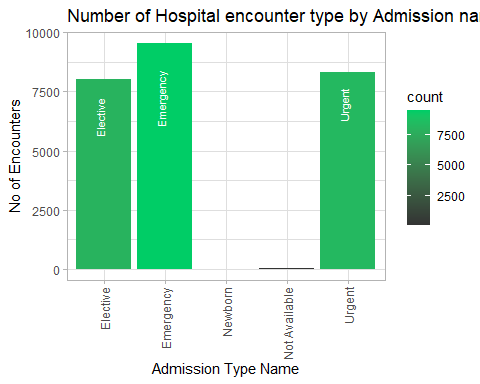
\includegraphics{Final_project_files/figure-latex/unnamed-chunk-1-1.pdf}

\begin{Shaded}
\begin{Highlighting}[]
\CommentTok{\# number of encounters by }
\NormalTok{diabetic  }\SpecialCharTok{\%\textgreater{}\%} \FunctionTok{group\_by}\NormalTok{(}\AttributeTok{specialty =}\NormalTok{ medical\_specialty) }\SpecialCharTok{\%\textgreater{}\%}
  \FunctionTok{summarise}\NormalTok{(}\AttributeTok{No\_of\_encounter =} \FunctionTok{n}\NormalTok{()) }\SpecialCharTok{\%\textgreater{}\%}
  \FunctionTok{arrange}\NormalTok{(}\FunctionTok{desc}\NormalTok{(No\_of\_encounter)) }\SpecialCharTok{\%\textgreater{}\%}
  \FunctionTok{top\_n}\NormalTok{(}\DecValTok{15}\NormalTok{, }\AttributeTok{wt =}\NormalTok{ No\_of\_encounter) }\SpecialCharTok{\%\textgreater{}\%} 
  \FunctionTok{ggplot}\NormalTok{(}\FunctionTok{aes}\NormalTok{(}\AttributeTok{x =}\NormalTok{ specialty, }\AttributeTok{y =}\NormalTok{ No\_of\_encounter, }\AttributeTok{fill =}\NormalTok{ No\_of\_encounter)) }\SpecialCharTok{+}
  \FunctionTok{geom\_bar}\NormalTok{(}\AttributeTok{position =} \StringTok{"dodge"}\NormalTok{, }\AttributeTok{stat=}\StringTok{"identity"}\NormalTok{)}\SpecialCharTok{+}
  \FunctionTok{scale\_fill\_gradient}\NormalTok{(}\AttributeTok{low =} \StringTok{"blue2"}\NormalTok{, }\AttributeTok{high =} \StringTok{"springgreen3"}\NormalTok{)}\SpecialCharTok{+}
  \FunctionTok{theme\_light}\NormalTok{()}\SpecialCharTok{+}
  \FunctionTok{theme}\NormalTok{(}\AttributeTok{axis.text.x =} \FunctionTok{element\_text}\NormalTok{(}\AttributeTok{angle =} \DecValTok{90}\NormalTok{, }\AttributeTok{vjust =} \FloatTok{0.5}\NormalTok{, }\AttributeTok{hjust =} \DecValTok{1}\NormalTok{))}\SpecialCharTok{+}\FunctionTok{labs}\NormalTok{(}\AttributeTok{height=}\DecValTok{10}\NormalTok{, }\AttributeTok{width=}\DecValTok{5}\NormalTok{)}\SpecialCharTok{+}
  \FunctionTok{coord\_flip}\NormalTok{() }\SpecialCharTok{+} \FunctionTok{labs}\NormalTok{(}\AttributeTok{title =} \StringTok{"Number of Hospital encounter Types by Specialty"}\NormalTok{, }\AttributeTok{x =} \StringTok{"Hospital Specialty"}\NormalTok{, }\AttributeTok{y =} \StringTok{"no of Encounters"}\NormalTok{)}
\end{Highlighting}
\end{Shaded}

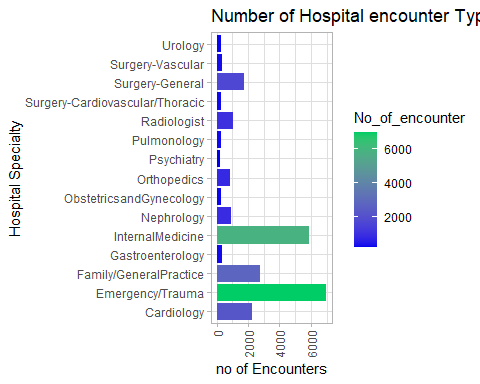
\includegraphics{Final_project_files/figure-latex/unnamed-chunk-1-2.pdf}

\begin{Shaded}
\begin{Highlighting}[]
\CommentTok{\# remove the icd 9 code to reveal more inormation }
  
\NormalTok{diabetic}\SpecialCharTok{$}\NormalTok{diag\_1 }\OtherTok{\textless{}{-}} \FunctionTok{str\_replace\_all}\NormalTok{(diabetic}\SpecialCharTok{$}\NormalTok{diag\_1, }\StringTok{"[[:punct:]]"}\NormalTok{, }\StringTok{""}\NormalTok{)}
\NormalTok{diabetic}\SpecialCharTok{$}\NormalTok{diag\_2 }\OtherTok{\textless{}{-}} \FunctionTok{str\_replace\_all}\NormalTok{(diabetic}\SpecialCharTok{$}\NormalTok{diag\_2, }\StringTok{"[[:punct:]]"}\NormalTok{, }\StringTok{""}\NormalTok{)}
\NormalTok{diabetic}\SpecialCharTok{$}\NormalTok{diag\_3 }\OtherTok{\textless{}{-}} \FunctionTok{str\_replace\_all}\NormalTok{(diabetic}\SpecialCharTok{$}\NormalTok{diag\_3, }\StringTok{"[[:punct:]]"}\NormalTok{, }\StringTok{""}\NormalTok{)}

\CommentTok{\# read the icd 9 code from }
\NormalTok{icd\_9 }\OtherTok{\textless{}{-}} \FunctionTok{read.delim}\NormalTok{(}\StringTok{"https://raw.githubusercontent.com/joewarner89/CUNY{-}607/main/Final\%20Project/icd9.txt"}\NormalTok{,}\AttributeTok{stringsAsFactors =}\NormalTok{ F) }\SpecialCharTok{\%\textgreater{}\%} \FunctionTok{rename}\NormalTok{(}\AttributeTok{diag\_1 =} \DecValTok{1}\NormalTok{,}\AttributeTok{Short\_desc =} \DecValTok{3}\NormalTok{)}
\end{Highlighting}
\end{Shaded}

The risk of developing pneumonia increase with diabetes. According to
healthline.com, diabetes weaken your immune system. In our data set, we
have 908 Hospital visits that result in a claim for pneumonia and about
185 for population ages 18 years and older that was diagnosed with
uncontrolled diabetes. We may have more patients that fits these
diagnosis.

The data do not contain any diagnosis name and group name. We download
the ICD 9 code from CMS data and major name was collected in this link
\url{https://juniperpublishers.com/ctbeb/CTBEB.MS.ID.555715.php}

The next step is to create diagnosis category to capture all major
events. see picture below:

\begin{figure}
\centering
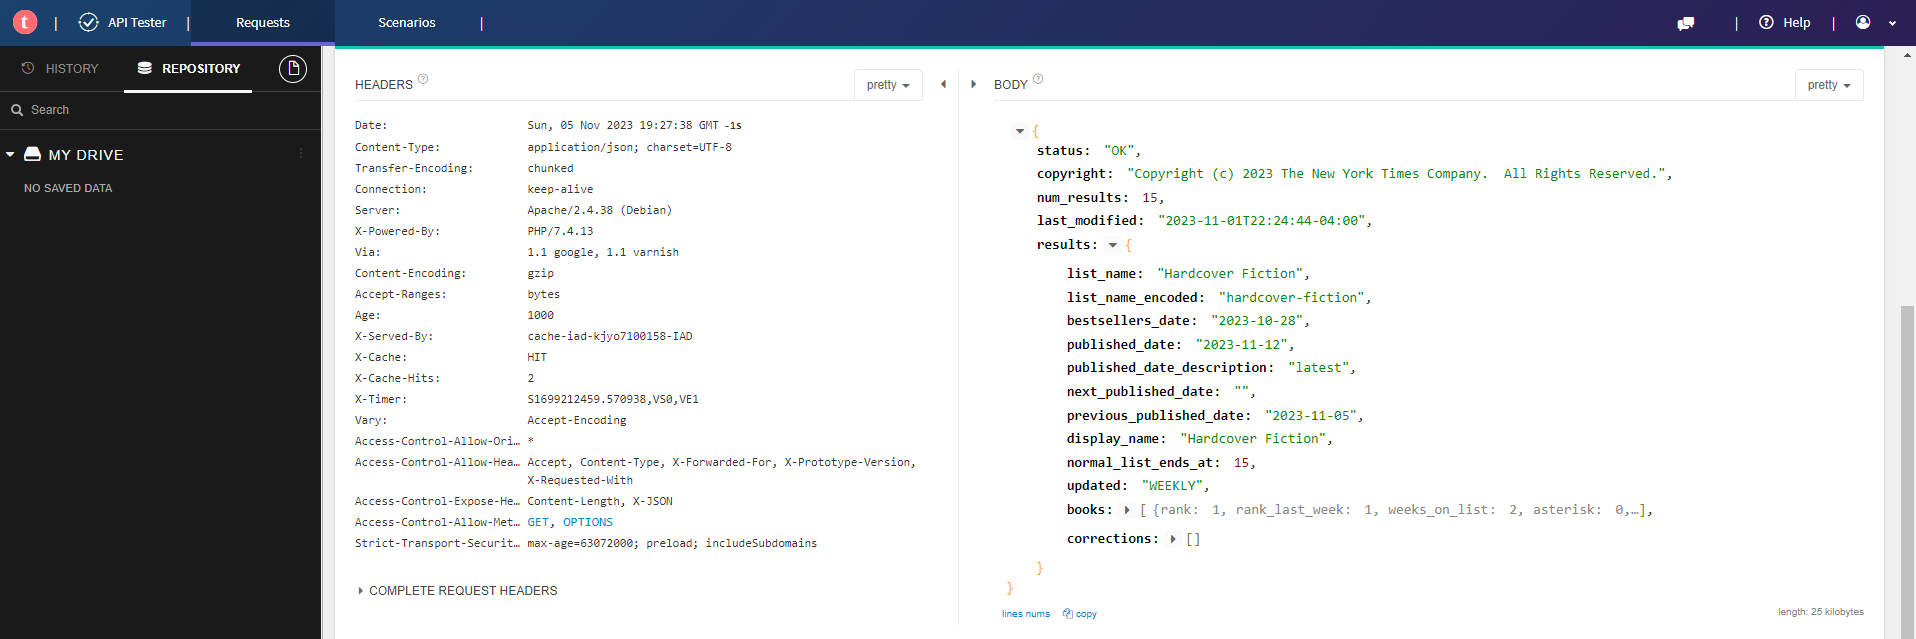
\includegraphics{C:/Users/Warner_Beast/OneDrive/Documents/CUNY/DATA 607 - Data Acquisition and Management/Final Project/Screenshot.png}
\caption{Main Group Name for ICD 9}
\end{figure}

\begin{Shaded}
\begin{Highlighting}[]
\CommentTok{\# look at the main diagnosis for }

\NormalTok{diabetic   }\SpecialCharTok{\%\textgreater{}\%}
  \FunctionTok{inner\_join}\NormalTok{(icd\_9,}\AttributeTok{by=}\StringTok{"diag\_1"}\NormalTok{)  }\SpecialCharTok{\%\textgreater{}\%} \FunctionTok{select}\NormalTok{(encounter\_id,diag\_1,Short\_desc) }\SpecialCharTok{\%\textgreater{}\%} 
  \FunctionTok{group\_by}\NormalTok{(Short\_desc) }\SpecialCharTok{\%\textgreater{}\%}  \FunctionTok{summarize}\NormalTok{(}\AttributeTok{No\_of\_encounter =} \FunctionTok{n}\NormalTok{()) }\SpecialCharTok{\%\textgreater{}\%} 
  \FunctionTok{arrange}\NormalTok{(}\FunctionTok{desc}\NormalTok{(No\_of\_encounter)) }\SpecialCharTok{\%\textgreater{}\%}
  \FunctionTok{top\_n}\NormalTok{(}\DecValTok{15}\NormalTok{, }\AttributeTok{wt =}\NormalTok{ No\_of\_encounter) }\SpecialCharTok{\%\textgreater{}\%}
  \FunctionTok{ggplot}\NormalTok{(}\FunctionTok{aes}\NormalTok{(}\AttributeTok{x =}\NormalTok{ Short\_desc, }\AttributeTok{y =}\NormalTok{ No\_of\_encounter, }\AttributeTok{fill =}\NormalTok{ No\_of\_encounter)) }\SpecialCharTok{+}
  \FunctionTok{geom\_bar}\NormalTok{(}\AttributeTok{position =} \StringTok{"dodge"}\NormalTok{, }\AttributeTok{stat=}\StringTok{"identity"}\NormalTok{)}\SpecialCharTok{+}
  \FunctionTok{scale\_fill\_gradient}\NormalTok{(}\AttributeTok{low =} \StringTok{"blue2"}\NormalTok{, }\AttributeTok{high =} \StringTok{"springgreen3"}\NormalTok{)}\SpecialCharTok{+}
  \FunctionTok{theme\_light}\NormalTok{()}\SpecialCharTok{+}
  \FunctionTok{theme}\NormalTok{(}\AttributeTok{axis.text.x =} \FunctionTok{element\_text}\NormalTok{(}\AttributeTok{angle =} \DecValTok{90}\NormalTok{, }\AttributeTok{vjust =} \FloatTok{0.5}\NormalTok{, }\AttributeTok{hjust =} \DecValTok{1}\NormalTok{))}\SpecialCharTok{+}\FunctionTok{labs}\NormalTok{(}\AttributeTok{height=}\DecValTok{10}\NormalTok{, }\AttributeTok{width=}\DecValTok{5}\NormalTok{)}\SpecialCharTok{+}
  \FunctionTok{coord\_flip}\NormalTok{() }\SpecialCharTok{+} \FunctionTok{labs}\NormalTok{(}\AttributeTok{title =} \StringTok{"Number of Hospital Diagnosis by ICD 9"}\NormalTok{, }\AttributeTok{x =} \StringTok{"ICD 9 Name"}\NormalTok{, }\AttributeTok{y =} \StringTok{"no of Encounters"}\NormalTok{)}
\end{Highlighting}
\end{Shaded}

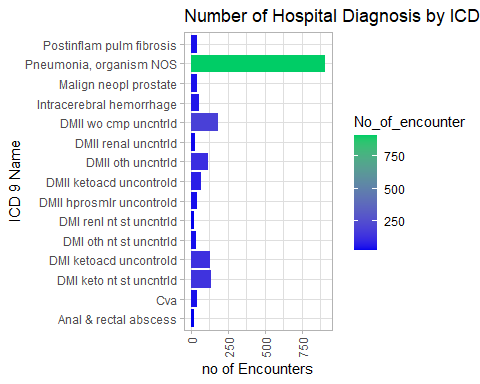
\includegraphics{Final_project_files/figure-latex/unnamed-chunk-2-1.pdf}

\begin{Shaded}
\begin{Highlighting}[]
\CommentTok{\# Diabetes Poor controls}
\NormalTok{diag\_cate }\OtherTok{\textless{}{-}} \FunctionTok{c}\NormalTok{(}\StringTok{"2511"}\NormalTok{, }\StringTok{"2512"}\NormalTok{, }\StringTok{"24901"}\NormalTok{, }\StringTok{"24930"}\NormalTok{, }\StringTok{"24931"}\NormalTok{, }\StringTok{"24941"}\NormalTok{, }\StringTok{"24951"}\NormalTok{,}\StringTok{" 24961"}\NormalTok{, }\StringTok{\textquotesingle{}24971\textquotesingle{}}\NormalTok{, }\StringTok{"24981"}\NormalTok{, }\StringTok{"24991"}\NormalTok{, }\StringTok{"25002"}\NormalTok{, }\StringTok{"25003"}\NormalTok{, }\StringTok{"25030"}\NormalTok{, }\StringTok{"25031"}\NormalTok{,}
               \StringTok{"25032"}\NormalTok{, }\StringTok{"25033"}\NormalTok{, }\StringTok{"25042"}\NormalTok{, }\StringTok{"25043,"}\NormalTok{, }\StringTok{"25052"}\NormalTok{, }\StringTok{"25053"}\NormalTok{, }\StringTok{"25062"}\NormalTok{, }\StringTok{"25063"}\NormalTok{, }\StringTok{"25072"}\NormalTok{, }\StringTok{"25073"}\NormalTok{, }\StringTok{"25082"}\NormalTok{, }\StringTok{"25083"}\NormalTok{, }\StringTok{"25092"}\NormalTok{, }\StringTok{"25093"}\NormalTok{)}

\CommentTok{\# Create diagnosis table }
\NormalTok{data }\OtherTok{\textless{}{-}} \FunctionTok{mutate}\NormalTok{(diabetic, }\AttributeTok{diagnosis =}
         \FunctionTok{ifelse}\NormalTok{(}\FunctionTok{str\_detect}\NormalTok{(diag\_1, }\StringTok{"V"}\NormalTok{) }\SpecialCharTok{|} \FunctionTok{str\_detect}\NormalTok{(diag\_1, }\StringTok{"E"}\NormalTok{),}\StringTok{"Other"}\NormalTok{, }
                \CommentTok{\# disease codes starting with V or E are in “other” category;}
                \FunctionTok{ifelse}\NormalTok{(}\FunctionTok{str\_detect}\NormalTok{(diag\_1, }\StringTok{"250"}\NormalTok{), }\StringTok{"Diabetes"}\NormalTok{,}
                       \FunctionTok{ifelse}\NormalTok{((}\FunctionTok{as.integer}\NormalTok{(diag\_1) }\SpecialCharTok{\%in\%}\NormalTok{ diag\_cate }\SpecialCharTok{\&} \FunctionTok{as.integer}\NormalTok{(diag\_1) }\SpecialCharTok{\textless{}=} \DecValTok{459}\NormalTok{) }\SpecialCharTok{|} \FunctionTok{as.integer}\NormalTok{(diag\_1) }\SpecialCharTok{==} \DecValTok{785}\NormalTok{, }\StringTok{"Circulatory"}\NormalTok{,}
                              \FunctionTok{ifelse}\NormalTok{((}\FunctionTok{as.integer}\NormalTok{(diag\_1) }\SpecialCharTok{\textgreater{}=} \DecValTok{460} \SpecialCharTok{\&} \FunctionTok{as.integer}\NormalTok{(diag\_1) }\SpecialCharTok{\textless{}=} \DecValTok{519}\NormalTok{) }\SpecialCharTok{|} \FunctionTok{as.integer}\NormalTok{(diag\_1) }\SpecialCharTok{==} \DecValTok{786}\NormalTok{, }\StringTok{"Respiratory"}\NormalTok{, }
                                     \FunctionTok{ifelse}\NormalTok{((}\FunctionTok{as.integer}\NormalTok{(diag\_1) }\SpecialCharTok{\textgreater{}=} \DecValTok{520} \SpecialCharTok{\&} \FunctionTok{as.integer}\NormalTok{(diag\_1) }\SpecialCharTok{\textless{}=} \DecValTok{579}\NormalTok{) }\SpecialCharTok{|} \FunctionTok{as.integer}\NormalTok{(diag\_1) }\SpecialCharTok{==} \DecValTok{787}\NormalTok{, }\StringTok{"Digestive"}\NormalTok{, }
                                            \FunctionTok{ifelse}\NormalTok{((}\FunctionTok{as.integer}\NormalTok{(diag\_1) }\SpecialCharTok{\textgreater{}=} \DecValTok{580} \SpecialCharTok{\&} \FunctionTok{as.integer}\NormalTok{(diag\_1) }\SpecialCharTok{\textless{}=} \DecValTok{629}\NormalTok{) }\SpecialCharTok{|} \FunctionTok{as.integer}\NormalTok{(diag\_1) }\SpecialCharTok{==} \DecValTok{788}\NormalTok{, }\StringTok{"Genitourinary"}\NormalTok{,}
                                                   \FunctionTok{ifelse}\NormalTok{((}\FunctionTok{as.integer}\NormalTok{(diag\_1) }\SpecialCharTok{\textgreater{}=} \DecValTok{140} \SpecialCharTok{\&} \FunctionTok{as.integer}\NormalTok{(diag\_1) }\SpecialCharTok{\textless{}=} \DecValTok{239}\NormalTok{), }\StringTok{"Neoplasms"}\NormalTok{,  }
                                                          \FunctionTok{ifelse}\NormalTok{((}\FunctionTok{as.integer}\NormalTok{(diag\_1) }\SpecialCharTok{\textgreater{}=} \DecValTok{710} \SpecialCharTok{\&} \FunctionTok{as.integer}\NormalTok{(diag\_1) }\SpecialCharTok{\textless{}=} \DecValTok{739}\NormalTok{), }\StringTok{"Musculoskeletal"}\NormalTok{,          }
                                                                 \FunctionTok{ifelse}\NormalTok{((}\FunctionTok{as.integer}\NormalTok{(diag\_1) }\SpecialCharTok{\textgreater{}=} \DecValTok{800} \SpecialCharTok{\&} \FunctionTok{as.integer}\NormalTok{(diag\_1) }\SpecialCharTok{\textless{}=} \DecValTok{999}\NormalTok{), }\StringTok{"Injury"}\NormalTok{,                    }
                                                                        \StringTok{"Circulatory"}\NormalTok{))))))))))}


\CommentTok{\# Group Name by encounter count}

\NormalTok{data }\SpecialCharTok{\%\textgreater{}\%}  \FunctionTok{group\_by}\NormalTok{(diagnosis,race) }\SpecialCharTok{\%\textgreater{}\%} \FunctionTok{summarise}\NormalTok{(}\AttributeTok{count =} \FunctionTok{n}\NormalTok{()) }\SpecialCharTok{\%\textgreater{}\%} \FunctionTok{group\_by}\NormalTok{(diagnosis) }\SpecialCharTok{\%\textgreater{}\%}
  \FunctionTok{ggplot}\NormalTok{(}\FunctionTok{aes}\NormalTok{(}\AttributeTok{x =}\NormalTok{diagnosis, }\AttributeTok{y =}\NormalTok{ count, }\AttributeTok{fill =}\NormalTok{ race)) }\SpecialCharTok{+}
  \FunctionTok{geom\_col}\NormalTok{() }\SpecialCharTok{+}
   \FunctionTok{labs}\NormalTok{(}\AttributeTok{title =} \StringTok{"Number of Hospital encounter Types by Diagnosis Group"}\NormalTok{, }\AttributeTok{x =} \StringTok{"Group Name"}\NormalTok{, }\AttributeTok{y =} \StringTok{"no of Encounters"}\NormalTok{)}
\end{Highlighting}
\end{Shaded}

\begin{verbatim}
## `summarise()` has grouped output by 'diagnosis'. You can override using the
## `.groups` argument.
\end{verbatim}

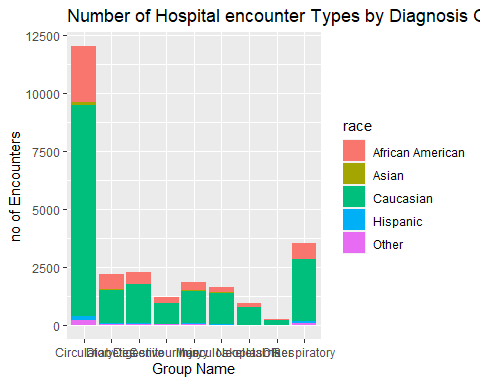
\includegraphics{Final_project_files/figure-latex/unnamed-chunk-2-2.pdf}

\begin{Shaded}
\begin{Highlighting}[]
\CommentTok{\# Number of men and women affected by diabetes }
\NormalTok{data }\SpecialCharTok{\%\textgreater{}\%}  \FunctionTok{group\_by}\NormalTok{(race,gender) }\SpecialCharTok{\%\textgreater{}\%} \FunctionTok{summarise}\NormalTok{(}\AttributeTok{count =} \FunctionTok{n}\NormalTok{()) }\SpecialCharTok{\%\textgreater{}\%}  \FunctionTok{arrange}\NormalTok{(}\FunctionTok{desc}\NormalTok{(count)) }\SpecialCharTok{\%\textgreater{}\%}
  \FunctionTok{ggplot}\NormalTok{(}\FunctionTok{aes}\NormalTok{(}\AttributeTok{x =}\NormalTok{race, }\AttributeTok{y =}\NormalTok{ count, }\AttributeTok{fill =}\NormalTok{ gender)) }\SpecialCharTok{+}
  \FunctionTok{geom\_col}\NormalTok{() }\SpecialCharTok{+}
  \FunctionTok{labs}\NormalTok{(}\AttributeTok{title =} \StringTok{"Number of Hospital encounter Types by Gender and Race"}\NormalTok{, }\AttributeTok{x =} \StringTok{"Group Name"}\NormalTok{, }\AttributeTok{y =} \StringTok{"no of Encounters"}\NormalTok{)}
\end{Highlighting}
\end{Shaded}

\begin{verbatim}
## `summarise()` has grouped output by 'race'. You can override using the
## `.groups` argument.
\end{verbatim}

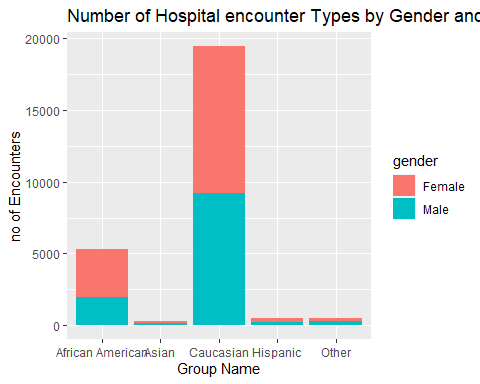
\includegraphics{Final_project_files/figure-latex/unnamed-chunk-2-3.pdf}

\begin{Shaded}
\begin{Highlighting}[]
\CommentTok{\# gender stats }

\NormalTok{gender\_stat }\OtherTok{\textless{}{-}}\NormalTok{ data }\SpecialCharTok{\%\textgreater{}\%}  \FunctionTok{group\_by}\NormalTok{(race,gender) }\SpecialCharTok{\%\textgreater{}\%} \FunctionTok{summarise}\NormalTok{(}\AttributeTok{count =} \FunctionTok{n}\NormalTok{()) }\SpecialCharTok{\%\textgreater{}\%}  \FunctionTok{arrange}\NormalTok{(}\FunctionTok{desc}\NormalTok{(count))}
\end{Highlighting}
\end{Shaded}

\begin{verbatim}
## `summarise()` has grouped output by 'race'. You can override using the
## `.groups` argument.
\end{verbatim}

\begin{Shaded}
\begin{Highlighting}[]
\FunctionTok{htmlTable}\NormalTok{(gender\_stat)}
\end{Highlighting}
\end{Shaded}

race

gender

count

1

Caucasian

Female

10221

2

Caucasian

Male

9240

3

African American

Female

3307

4

African American

Male

1980

5

Other

Male

247

6

Hispanic

Female

237

7

Hispanic

Male

227

8

Other

Female

218

9

Asian

Male

130

10

Asian

Female

119

Diabetes mellitus or diabetes disproportionately affects minority
populations. Most patients who poor control over their diabetes
treatment face circulatory issues. In the data set, both caucasian and
African american have the high number of circulatory diagnosis. There
are more women caucasian that are diagnosed with diabetes more than
every ethnic group.

\hypertarget{multivariate-and-univariate-analysis}{%
\subsection{Multivariate and Univariate
Analysis}\label{multivariate-and-univariate-analysis}}

We modify the input of some the features to scale the data set. I make
change to some categorical values. This data set has more than 15
categorical values. It is very useful to understand the impact of each
variables in real life. Medication play a big part of treatments for
Diabetes. Some of the features present a challenge due to the way they
were created. Variables with low variances are not reliable for
statistical modeling.

We combine all the low variance columns to add more variances to the
data and preserve the information. Based on the initial graph we did, we
need to remove outliers.

\begin{Shaded}
\begin{Highlighting}[]
\CommentTok{\# reassign data set }
\NormalTok{lib }\OtherTok{\textless{}{-}}\NormalTok{ data }

\DocumentationTok{\#\# Removing duplicate patients encounter}
\NormalTok{lib }\OtherTok{\textless{}{-}}\NormalTok{ lib[}\SpecialCharTok{!}\FunctionTok{duplicated}\NormalTok{(lib}\SpecialCharTok{$}\NormalTok{patient\_nbr),]}

\CommentTok{\# Change some categorical data to numerical}
\CommentTok{\# recategorize the column age}
\NormalTok{lib}\SpecialCharTok{$}\NormalTok{age }\OtherTok{\textless{}{-}} \FunctionTok{ifelse}\NormalTok{(lib}\SpecialCharTok{$}\NormalTok{age }\SpecialCharTok{==} \StringTok{"[0{-}10)"}\NormalTok{,  }\DecValTok{0}\NormalTok{, lib}\SpecialCharTok{$}\NormalTok{age);}
\NormalTok{lib}\SpecialCharTok{$}\NormalTok{age }\OtherTok{\textless{}{-}} \FunctionTok{ifelse}\NormalTok{(lib}\SpecialCharTok{$}\NormalTok{age }\SpecialCharTok{==} \StringTok{"[10{-}20)"}\NormalTok{, }\DecValTok{10}\NormalTok{, lib}\SpecialCharTok{$}\NormalTok{age);}
\NormalTok{lib}\SpecialCharTok{$}\NormalTok{age }\OtherTok{\textless{}{-}} \FunctionTok{ifelse}\NormalTok{(lib}\SpecialCharTok{$}\NormalTok{age }\SpecialCharTok{==} \StringTok{"[20{-}30)"}\NormalTok{, }\DecValTok{20}\NormalTok{, lib}\SpecialCharTok{$}\NormalTok{age);}
\NormalTok{lib}\SpecialCharTok{$}\NormalTok{age }\OtherTok{\textless{}{-}} \FunctionTok{ifelse}\NormalTok{(lib}\SpecialCharTok{$}\NormalTok{age }\SpecialCharTok{==} \StringTok{"[30{-}40)"}\NormalTok{, }\DecValTok{30}\NormalTok{, lib}\SpecialCharTok{$}\NormalTok{age);}
\NormalTok{lib}\SpecialCharTok{$}\NormalTok{age }\OtherTok{\textless{}{-}} \FunctionTok{ifelse}\NormalTok{(lib}\SpecialCharTok{$}\NormalTok{age }\SpecialCharTok{==} \StringTok{"[40{-}50)"}\NormalTok{, }\DecValTok{40}\NormalTok{, lib}\SpecialCharTok{$}\NormalTok{age);}
\NormalTok{lib}\SpecialCharTok{$}\NormalTok{age }\OtherTok{\textless{}{-}} \FunctionTok{ifelse}\NormalTok{(lib}\SpecialCharTok{$}\NormalTok{age }\SpecialCharTok{==} \StringTok{"[50{-}60)"}\NormalTok{, }\DecValTok{50}\NormalTok{, lib}\SpecialCharTok{$}\NormalTok{age);}
\NormalTok{lib}\SpecialCharTok{$}\NormalTok{age }\OtherTok{\textless{}{-}} \FunctionTok{ifelse}\NormalTok{(lib}\SpecialCharTok{$}\NormalTok{age }\SpecialCharTok{==} \StringTok{"[60{-}70)"}\NormalTok{, }\DecValTok{60}\NormalTok{, lib}\SpecialCharTok{$}\NormalTok{age);}
\NormalTok{lib}\SpecialCharTok{$}\NormalTok{age }\OtherTok{\textless{}{-}} \FunctionTok{ifelse}\NormalTok{(lib}\SpecialCharTok{$}\NormalTok{age }\SpecialCharTok{==} \StringTok{"[70{-}80)"}\NormalTok{, }\DecValTok{70}\NormalTok{, lib}\SpecialCharTok{$}\NormalTok{age);}
\NormalTok{lib}\SpecialCharTok{$}\NormalTok{age }\OtherTok{\textless{}{-}} \FunctionTok{ifelse}\NormalTok{(lib}\SpecialCharTok{$}\NormalTok{age }\SpecialCharTok{==} \StringTok{"[80{-}90)"}\NormalTok{, }\DecValTok{80}\NormalTok{, lib}\SpecialCharTok{$}\NormalTok{age);}
\NormalTok{lib}\SpecialCharTok{$}\NormalTok{age }\OtherTok{\textless{}{-}} \FunctionTok{ifelse}\NormalTok{(lib}\SpecialCharTok{$}\NormalTok{age }\SpecialCharTok{==} \StringTok{"[90{-}100)"}\NormalTok{, }\DecValTok{90}\NormalTok{, lib}\SpecialCharTok{$}\NormalTok{age);}

\CommentTok{\# Change categorical values }
\NormalTok{lib}\SpecialCharTok{$}\NormalTok{max\_glu\_serum }\OtherTok{\textless{}{-}} \FunctionTok{ifelse}\NormalTok{(lib}\SpecialCharTok{$}\NormalTok{max\_glu\_serum }\SpecialCharTok{==} \StringTok{"None"}\NormalTok{,  }\DecValTok{0}\NormalTok{, lib}\SpecialCharTok{$}\NormalTok{max\_glu\_serum);}
\NormalTok{lib}\SpecialCharTok{$}\NormalTok{max\_glu\_serum }\OtherTok{\textless{}{-}} \FunctionTok{ifelse}\NormalTok{(lib}\SpecialCharTok{$}\NormalTok{max\_glu\_serum }\SpecialCharTok{==} \StringTok{"Norm"}\NormalTok{,  }\DecValTok{100}\NormalTok{, lib}\SpecialCharTok{$}\NormalTok{max\_glu\_serum);}
\NormalTok{lib}\SpecialCharTok{$}\NormalTok{max\_glu\_serum }\OtherTok{\textless{}{-}} \FunctionTok{ifelse}\NormalTok{(lib}\SpecialCharTok{$}\NormalTok{max\_glu\_serum }\SpecialCharTok{==} \StringTok{"\textgreater{}200"}\NormalTok{,  }\DecValTok{200}\NormalTok{, lib}\SpecialCharTok{$}\NormalTok{max\_glu\_serum);}
\NormalTok{lib}\SpecialCharTok{$}\NormalTok{max\_glu\_serum }\OtherTok{\textless{}{-}} \FunctionTok{ifelse}\NormalTok{(lib}\SpecialCharTok{$}\NormalTok{max\_glu\_serum }\SpecialCharTok{==} \StringTok{"\textgreater{}300"}\NormalTok{,  }\DecValTok{300}\NormalTok{, lib}\SpecialCharTok{$}\NormalTok{max\_glu\_serum);}

\NormalTok{lib}\SpecialCharTok{$}\NormalTok{A1Cresult }\OtherTok{\textless{}{-}} \FunctionTok{ifelse}\NormalTok{(lib}\SpecialCharTok{$}\NormalTok{A1Cresult }\SpecialCharTok{==} \StringTok{"None"}\NormalTok{,  }\DecValTok{0}\NormalTok{, lib}\SpecialCharTok{$}\NormalTok{A1Cresult);}
\NormalTok{lib}\SpecialCharTok{$}\NormalTok{A1Cresult }\OtherTok{\textless{}{-}} \FunctionTok{ifelse}\NormalTok{(lib}\SpecialCharTok{$}\NormalTok{A1Cresult }\SpecialCharTok{==} \StringTok{"Norm"}\NormalTok{,  }\DecValTok{5}\NormalTok{, lib}\SpecialCharTok{$}\NormalTok{A1Cresult);}
\NormalTok{lib}\SpecialCharTok{$}\NormalTok{A1Cresult }\OtherTok{\textless{}{-}} \FunctionTok{ifelse}\NormalTok{(lib}\SpecialCharTok{$}\NormalTok{A1Cresult }\SpecialCharTok{==} \StringTok{"\textgreater{}7"}\NormalTok{,    }\DecValTok{7}\NormalTok{, lib}\SpecialCharTok{$}\NormalTok{A1Cresult);}
\NormalTok{lib}\SpecialCharTok{$}\NormalTok{A1Cresult }\OtherTok{\textless{}{-}} \FunctionTok{ifelse}\NormalTok{(lib}\SpecialCharTok{$}\NormalTok{A1Cresult }\SpecialCharTok{==} \StringTok{"\textgreater{}8"}\NormalTok{,    }\DecValTok{8}\NormalTok{, lib}\SpecialCharTok{$}\NormalTok{A1Cresult);}

\NormalTok{lib}\SpecialCharTok{$}\NormalTok{metformin }\OtherTok{\textless{}{-}} \FunctionTok{ifelse}\NormalTok{(lib}\SpecialCharTok{$}\NormalTok{metformin }\SpecialCharTok{==} \StringTok{\textquotesingle{}No\textquotesingle{}}\NormalTok{, }\DecValTok{0}\NormalTok{ , lib}\SpecialCharTok{$}\NormalTok{metformin);}
\NormalTok{lib}\SpecialCharTok{$}\NormalTok{metformin }\OtherTok{\textless{}{-}} \FunctionTok{ifelse}\NormalTok{(lib}\SpecialCharTok{$}\NormalTok{metformin }\SpecialCharTok{==} \StringTok{\textquotesingle{}Steady\textquotesingle{}}\NormalTok{, }\DecValTok{1}\NormalTok{ , lib}\SpecialCharTok{$}\NormalTok{metformin);}
\NormalTok{lib}\SpecialCharTok{$}\NormalTok{metformin }\OtherTok{\textless{}{-}} \FunctionTok{ifelse}\NormalTok{(lib}\SpecialCharTok{$}\NormalTok{metformin }\SpecialCharTok{==} \StringTok{\textquotesingle{}Up\textquotesingle{}}\NormalTok{, }\DecValTok{2}\NormalTok{ , lib}\SpecialCharTok{$}\NormalTok{metformin);}
\NormalTok{lib}\SpecialCharTok{$}\NormalTok{metformin }\OtherTok{\textless{}{-}} \FunctionTok{ifelse}\NormalTok{(lib}\SpecialCharTok{$}\NormalTok{metformin }\SpecialCharTok{==} \StringTok{\textquotesingle{}Down\textquotesingle{}}\NormalTok{, }\DecValTok{3}\NormalTok{ , lib}\SpecialCharTok{$}\NormalTok{metformin);}

\NormalTok{lib}\SpecialCharTok{$}\NormalTok{repaglinide }\OtherTok{\textless{}{-}} \FunctionTok{ifelse}\NormalTok{(lib}\SpecialCharTok{$}\NormalTok{repaglinide }\SpecialCharTok{==} \StringTok{\textquotesingle{}No\textquotesingle{}}\NormalTok{, }\DecValTok{0}\NormalTok{ , lib}\SpecialCharTok{$}\NormalTok{repaglinide);}
\NormalTok{lib}\SpecialCharTok{$}\NormalTok{repaglinide }\OtherTok{\textless{}{-}} \FunctionTok{ifelse}\NormalTok{(lib}\SpecialCharTok{$}\NormalTok{repaglinide }\SpecialCharTok{==} \StringTok{\textquotesingle{}Steady\textquotesingle{}}\NormalTok{, }\DecValTok{1}\NormalTok{ , lib}\SpecialCharTok{$}\NormalTok{repaglinide);}
\NormalTok{lib}\SpecialCharTok{$}\NormalTok{repaglinide }\OtherTok{\textless{}{-}} \FunctionTok{ifelse}\NormalTok{(lib}\SpecialCharTok{$}\NormalTok{repaglinide }\SpecialCharTok{==} \StringTok{\textquotesingle{}Up\textquotesingle{}}\NormalTok{, }\DecValTok{2}\NormalTok{ , lib}\SpecialCharTok{$}\NormalTok{repaglinide);}
\NormalTok{lib}\SpecialCharTok{$}\NormalTok{repaglinide }\OtherTok{\textless{}{-}} \FunctionTok{ifelse}\NormalTok{(lib}\SpecialCharTok{$}\NormalTok{repaglinide }\SpecialCharTok{==} \StringTok{\textquotesingle{}Down\textquotesingle{}}\NormalTok{, }\DecValTok{3}\NormalTok{ , lib}\SpecialCharTok{$}\NormalTok{repaglinide);}

\NormalTok{lib}\SpecialCharTok{$}\NormalTok{chlorpropamide }\OtherTok{\textless{}{-}} \FunctionTok{ifelse}\NormalTok{(lib}\SpecialCharTok{$}\NormalTok{chlorpropamide }\SpecialCharTok{==} \StringTok{\textquotesingle{}No\textquotesingle{}}\NormalTok{, }\DecValTok{0}\NormalTok{ , lib}\SpecialCharTok{$}\NormalTok{chlorpropamide);}
\NormalTok{lib}\SpecialCharTok{$}\NormalTok{chlorpropamide }\OtherTok{\textless{}{-}} \FunctionTok{ifelse}\NormalTok{(lib}\SpecialCharTok{$}\NormalTok{chlorpropamide }\SpecialCharTok{==} \StringTok{\textquotesingle{}Steady\textquotesingle{}}\NormalTok{, }\DecValTok{1}\NormalTok{ , lib}\SpecialCharTok{$}\NormalTok{chlorpropamide);}
\NormalTok{lib}\SpecialCharTok{$}\NormalTok{chlorpropamide }\OtherTok{\textless{}{-}} \FunctionTok{ifelse}\NormalTok{(lib}\SpecialCharTok{$}\NormalTok{chlorpropamide }\SpecialCharTok{==} \StringTok{\textquotesingle{}Up\textquotesingle{}}\NormalTok{, }\DecValTok{2}\NormalTok{ , lib}\SpecialCharTok{$}\NormalTok{chlorpropamide);}
\NormalTok{lib}\SpecialCharTok{$}\NormalTok{chlorpropamide }\OtherTok{\textless{}{-}} \FunctionTok{ifelse}\NormalTok{(lib}\SpecialCharTok{$}\NormalTok{chlorpropamide }\SpecialCharTok{==} \StringTok{\textquotesingle{}Down\textquotesingle{}}\NormalTok{, }\DecValTok{3}\NormalTok{ , lib}\SpecialCharTok{$}\NormalTok{chlorpropamide);}

\NormalTok{lib}\SpecialCharTok{$}\NormalTok{nateglinide }\OtherTok{\textless{}{-}} \FunctionTok{ifelse}\NormalTok{(lib}\SpecialCharTok{$}\NormalTok{nateglinide }\SpecialCharTok{==} \StringTok{\textquotesingle{}No\textquotesingle{}}\NormalTok{, }\DecValTok{0}\NormalTok{ , lib}\SpecialCharTok{$}\NormalTok{nateglinide);}
\NormalTok{lib}\SpecialCharTok{$}\NormalTok{nateglinide }\OtherTok{\textless{}{-}} \FunctionTok{ifelse}\NormalTok{(lib}\SpecialCharTok{$}\NormalTok{nateglinide }\SpecialCharTok{==} \StringTok{\textquotesingle{}Steady\textquotesingle{}}\NormalTok{, }\DecValTok{1}\NormalTok{ , lib}\SpecialCharTok{$}\NormalTok{nateglinide);}

\NormalTok{lib}\SpecialCharTok{$}\NormalTok{glimepiride }\OtherTok{\textless{}{-}} \FunctionTok{ifelse}\NormalTok{(lib}\SpecialCharTok{$}\NormalTok{glimepiride }\SpecialCharTok{==} \StringTok{\textquotesingle{}No\textquotesingle{}}\NormalTok{, }\DecValTok{0}\NormalTok{ , lib}\SpecialCharTok{$}\NormalTok{glimepiride);}
\NormalTok{lib}\SpecialCharTok{$}\NormalTok{glimepiride }\OtherTok{\textless{}{-}} \FunctionTok{ifelse}\NormalTok{(lib}\SpecialCharTok{$}\NormalTok{glimepiride }\SpecialCharTok{==} \StringTok{\textquotesingle{}Steady\textquotesingle{}}\NormalTok{, }\DecValTok{1}\NormalTok{ , lib}\SpecialCharTok{$}\NormalTok{glimepiride);}
\NormalTok{lib}\SpecialCharTok{$}\NormalTok{glimepiride }\OtherTok{\textless{}{-}} \FunctionTok{ifelse}\NormalTok{(lib}\SpecialCharTok{$}\NormalTok{glimepiride }\SpecialCharTok{==} \StringTok{\textquotesingle{}Up\textquotesingle{}}\NormalTok{, }\DecValTok{2}\NormalTok{ , lib}\SpecialCharTok{$}\NormalTok{glimepiride);}

\NormalTok{lib}\SpecialCharTok{$}\NormalTok{pioglitazone }\OtherTok{\textless{}{-}} \FunctionTok{ifelse}\NormalTok{(lib}\SpecialCharTok{$}\NormalTok{pioglitazone }\SpecialCharTok{==} \StringTok{\textquotesingle{}No\textquotesingle{}}\NormalTok{, }\DecValTok{0}\NormalTok{ , lib}\SpecialCharTok{$}\NormalTok{pioglitazone);}
\NormalTok{lib}\SpecialCharTok{$}\NormalTok{pioglitazone }\OtherTok{\textless{}{-}} \FunctionTok{ifelse}\NormalTok{(lib}\SpecialCharTok{$}\NormalTok{pioglitazone }\SpecialCharTok{==} \StringTok{\textquotesingle{}Steady\textquotesingle{}}\NormalTok{, }\DecValTok{1}\NormalTok{ , lib}\SpecialCharTok{$}\NormalTok{pioglitazone);}
\NormalTok{lib}\SpecialCharTok{$}\NormalTok{pioglitazone }\OtherTok{\textless{}{-}} \FunctionTok{ifelse}\NormalTok{(lib}\SpecialCharTok{$}\NormalTok{pioglitazone }\SpecialCharTok{==} \StringTok{\textquotesingle{}Up\textquotesingle{}}\NormalTok{, }\DecValTok{2}\NormalTok{ , lib}\SpecialCharTok{$}\NormalTok{pioglitazone);}

\NormalTok{lib}\SpecialCharTok{$}\NormalTok{glyburide }\OtherTok{\textless{}{-}} \FunctionTok{ifelse}\NormalTok{(lib}\SpecialCharTok{$}\NormalTok{glyburide }\SpecialCharTok{==} \StringTok{\textquotesingle{}No\textquotesingle{}}\NormalTok{, }\DecValTok{0}\NormalTok{ , lib}\SpecialCharTok{$}\NormalTok{glyburide);}
\NormalTok{lib}\SpecialCharTok{$}\NormalTok{glyburide }\OtherTok{\textless{}{-}} \FunctionTok{ifelse}\NormalTok{(lib}\SpecialCharTok{$}\NormalTok{glyburide }\SpecialCharTok{==} \StringTok{\textquotesingle{}Steady\textquotesingle{}}\NormalTok{, }\DecValTok{1}\NormalTok{ , lib}\SpecialCharTok{$}\NormalTok{glyburide);}
\NormalTok{lib}\SpecialCharTok{$}\NormalTok{glyburide }\OtherTok{\textless{}{-}} \FunctionTok{ifelse}\NormalTok{(lib}\SpecialCharTok{$}\NormalTok{glyburide }\SpecialCharTok{==} \StringTok{\textquotesingle{}Up\textquotesingle{}}\NormalTok{, }\DecValTok{2}\NormalTok{ , lib}\SpecialCharTok{$}\NormalTok{glyburide);}
\NormalTok{lib}\SpecialCharTok{$}\NormalTok{glyburide }\OtherTok{\textless{}{-}} \FunctionTok{ifelse}\NormalTok{(lib}\SpecialCharTok{$}\NormalTok{glyburide }\SpecialCharTok{==} \StringTok{\textquotesingle{}Down\textquotesingle{}}\NormalTok{, }\DecValTok{3}\NormalTok{ , lib}\SpecialCharTok{$}\NormalTok{glyburide);}

\NormalTok{lib}\SpecialCharTok{$}\NormalTok{acarbose }\OtherTok{\textless{}{-}} \FunctionTok{ifelse}\NormalTok{(lib}\SpecialCharTok{$}\NormalTok{acarbose }\SpecialCharTok{==} \StringTok{\textquotesingle{}No\textquotesingle{}}\NormalTok{, }\DecValTok{0}\NormalTok{ , lib}\SpecialCharTok{$}\NormalTok{acarbose);}
\NormalTok{lib}\SpecialCharTok{$}\NormalTok{acarbose }\OtherTok{\textless{}{-}} \FunctionTok{ifelse}\NormalTok{(lib}\SpecialCharTok{$}\NormalTok{acarbose }\SpecialCharTok{==} \StringTok{\textquotesingle{}Steady\textquotesingle{}}\NormalTok{, }\DecValTok{1}\NormalTok{ , lib}\SpecialCharTok{$}\NormalTok{acarbose);}

\NormalTok{lib}\SpecialCharTok{$}\NormalTok{insulin }\OtherTok{\textless{}{-}} \FunctionTok{ifelse}\NormalTok{(lib}\SpecialCharTok{$}\NormalTok{insulin }\SpecialCharTok{==} \StringTok{\textquotesingle{}No\textquotesingle{}}\NormalTok{, }\DecValTok{0}\NormalTok{ , lib}\SpecialCharTok{$}\NormalTok{insulin);}
\NormalTok{lib}\SpecialCharTok{$}\NormalTok{insulin }\OtherTok{\textless{}{-}} \FunctionTok{ifelse}\NormalTok{(lib}\SpecialCharTok{$}\NormalTok{insulin }\SpecialCharTok{==} \StringTok{\textquotesingle{}Steady\textquotesingle{}}\NormalTok{, }\DecValTok{1}\NormalTok{ , lib}\SpecialCharTok{$}\NormalTok{insulin);}
\NormalTok{lib}\SpecialCharTok{$}\NormalTok{insulin }\OtherTok{\textless{}{-}} \FunctionTok{ifelse}\NormalTok{(lib}\SpecialCharTok{$}\NormalTok{insulin }\SpecialCharTok{==} \StringTok{\textquotesingle{}Up\textquotesingle{}}\NormalTok{, }\DecValTok{2}\NormalTok{ , lib}\SpecialCharTok{$}\NormalTok{insulin);}
\NormalTok{lib}\SpecialCharTok{$}\NormalTok{insulin }\OtherTok{\textless{}{-}} \FunctionTok{ifelse}\NormalTok{(lib}\SpecialCharTok{$}\NormalTok{insulin }\SpecialCharTok{==} \StringTok{\textquotesingle{}Down\textquotesingle{}}\NormalTok{, }\DecValTok{3}\NormalTok{ , lib}\SpecialCharTok{$}\NormalTok{insulin);}

\NormalTok{lib}\SpecialCharTok{$}\NormalTok{glipizide.metformin }\OtherTok{\textless{}{-}} \FunctionTok{ifelse}\NormalTok{(lib}\SpecialCharTok{$}\NormalTok{glipizide.metformin }\SpecialCharTok{==} \StringTok{\textquotesingle{}No\textquotesingle{}}\NormalTok{, }\DecValTok{0}\NormalTok{ , lib}\SpecialCharTok{$}\NormalTok{glipizide.metformin);}
\NormalTok{lib}\SpecialCharTok{$}\NormalTok{glipizide.metformin }\OtherTok{\textless{}{-}} \FunctionTok{ifelse}\NormalTok{(lib}\SpecialCharTok{$}\NormalTok{glipizide.metformin }\SpecialCharTok{==} \StringTok{\textquotesingle{}Steady\textquotesingle{}}\NormalTok{, }\DecValTok{1}\NormalTok{ , lib}\SpecialCharTok{$}\NormalTok{glipizide.metformin);}

\NormalTok{lib}\SpecialCharTok{$}\NormalTok{change }\OtherTok{\textless{}{-}} \FunctionTok{ifelse}\NormalTok{(lib}\SpecialCharTok{$}\NormalTok{change }\SpecialCharTok{==} \StringTok{\textquotesingle{}No\textquotesingle{}}\NormalTok{, }\DecValTok{0}\NormalTok{ , lib}\SpecialCharTok{$}\NormalTok{change);}
\NormalTok{lib}\SpecialCharTok{$}\NormalTok{change }\OtherTok{\textless{}{-}} \FunctionTok{ifelse}\NormalTok{(lib}\SpecialCharTok{$}\NormalTok{change }\SpecialCharTok{==} \StringTok{\textquotesingle{}Ch\textquotesingle{}}\NormalTok{, }\DecValTok{1}\NormalTok{ , lib}\SpecialCharTok{$}\NormalTok{change);}

\NormalTok{lib}\SpecialCharTok{$}\NormalTok{diabetesMed }\OtherTok{\textless{}{-}} \FunctionTok{ifelse}\NormalTok{(lib}\SpecialCharTok{$}\NormalTok{diabetesMed }\SpecialCharTok{==} \StringTok{\textquotesingle{}No\textquotesingle{}}\NormalTok{, }\DecValTok{0}\NormalTok{ , lib}\SpecialCharTok{$}\NormalTok{diabetesMed);}
\NormalTok{lib}\SpecialCharTok{$}\NormalTok{diabetesMed }\OtherTok{\textless{}{-}} \FunctionTok{ifelse}\NormalTok{(lib}\SpecialCharTok{$}\NormalTok{diabetesMed }\SpecialCharTok{==} \StringTok{\textquotesingle{}Yes\textquotesingle{}}\NormalTok{, }\DecValTok{1}\NormalTok{ , lib}\SpecialCharTok{$}\NormalTok{diabetesMed);}
\CommentTok{\#See Variable with low variances }
\FunctionTok{nearZeroVar}\NormalTok{(lib, }\AttributeTok{names =}\NormalTok{ T, }\AttributeTok{freqCut =} \DecValTok{19}\NormalTok{, }\AttributeTok{uniqueCut =} \DecValTok{10}\NormalTok{)}
\end{Highlighting}
\end{Shaded}

\begin{verbatim}
##  [1] "max_glu_serum"          "repaglinide"            "nateglinide"           
##  [4] "chlorpropamide"         "acarbose"               "miglitol"              
##  [7] "tolazamide"             "glyburide.metformin"    "glipizide.metformin"   
## [10] "metformin.pioglitazone"
\end{verbatim}

\begin{Shaded}
\begin{Highlighting}[]
\CommentTok{\# re categorize encounter}
\CommentTok{\# Encounter is unique for every visit, so we are going create visit column to capture}
\CommentTok{\# the number of outpatient inpatient and emergency}

\NormalTok{lib}\SpecialCharTok{$}\NormalTok{visits }\OtherTok{=}\NormalTok{ lib}\SpecialCharTok{$}\NormalTok{number\_outpatient }\SpecialCharTok{+}\NormalTok{ lib}\SpecialCharTok{$}\NormalTok{number\_emergency }\SpecialCharTok{+}\NormalTok{ lib}\SpecialCharTok{$}\NormalTok{number\_inp}
\NormalTok{readmitted }\OtherTok{=}\NormalTok{ lib}\SpecialCharTok{$}\NormalTok{readmitted}
\NormalTok{lib }\OtherTok{\textless{}{-}} \FunctionTok{subset}\NormalTok{(lib, }\AttributeTok{select =}\SpecialCharTok{{-}}\FunctionTok{c}\NormalTok{(readmitted))}
\NormalTok{lib}\SpecialCharTok{$}\NormalTok{readmitted }\OtherTok{=}\NormalTok{ readmitted}

\CommentTok{\# identify low variance in the data set}
\CommentTok{\#This column has low variances }
\NormalTok{keys }\OtherTok{\textless{}{-}} \FunctionTok{nearZeroVar}\NormalTok{(lib, }\AttributeTok{names =}\NormalTok{ T, }\AttributeTok{freqCut =} \DecValTok{19}\NormalTok{, }\AttributeTok{uniqueCut =} \DecValTok{10}\NormalTok{)}
\NormalTok{keys}
\end{Highlighting}
\end{Shaded}

\begin{verbatim}
##  [1] "max_glu_serum"          "repaglinide"            "nateglinide"           
##  [4] "chlorpropamide"         "acarbose"               "miglitol"              
##  [7] "tolazamide"             "glyburide.metformin"    "glipizide.metformin"   
## [10] "metformin.pioglitazone"
\end{verbatim}

\begin{Shaded}
\begin{Highlighting}[]
\CommentTok{\# Low variance is usefull to identify outliers}
\CommentTok{\# correlation would be lower if variance is low.}
\NormalTok{lib}\SpecialCharTok{$}\NormalTok{num\_med }\OtherTok{\textless{}{-}} \DecValTok{0}
\NormalTok{lib}\SpecialCharTok{$}\NormalTok{num\_changes }\OtherTok{\textless{}{-}} \DecValTok{0}
\ControlFlowTok{for}\NormalTok{(key }\ControlFlowTok{in}\NormalTok{ keys)\{}
\NormalTok{  lib}\SpecialCharTok{$}\NormalTok{num\_med }\OtherTok{\textless{}{-}} \FunctionTok{ifelse}\NormalTok{(lib[key] }\SpecialCharTok{!=} \DecValTok{0}\NormalTok{, lib}\SpecialCharTok{$}\NormalTok{num\_med }\SpecialCharTok{+} \DecValTok{1}\NormalTok{, lib}\SpecialCharTok{$}\NormalTok{num\_med)}
\NormalTok{  lib}\SpecialCharTok{$}\NormalTok{num\_changes }\OtherTok{\textless{}{-}} \FunctionTok{ifelse}\NormalTok{((lib[key] }\SpecialCharTok{==} \DecValTok{1} \SpecialCharTok{|}\NormalTok{ lib[key] }\SpecialCharTok{==} \DecValTok{2} \SpecialCharTok{|}\NormalTok{ lib[key] }\SpecialCharTok{==} \DecValTok{3}\NormalTok{), lib}\SpecialCharTok{$}\NormalTok{num\_changes }\SpecialCharTok{+} \DecValTok{1}\NormalTok{, lib}\SpecialCharTok{$}\NormalTok{num\_changes)}
\NormalTok{\}}



\DocumentationTok{\#\# Normalize, Remove Outliers, and Standardize Numerical Features}
\NormalTok{lib}\SpecialCharTok{$}\NormalTok{number\_inpatient }\OtherTok{\textless{}{-}} \FunctionTok{log1p}\NormalTok{(lib}\SpecialCharTok{$}\NormalTok{number\_inpatient)}
\NormalTok{lib}\SpecialCharTok{$}\NormalTok{number\_outpatient }\OtherTok{\textless{}{-}} \FunctionTok{log1p}\NormalTok{(lib}\SpecialCharTok{$}\NormalTok{number\_outpatient)}
\NormalTok{lib}\SpecialCharTok{$}\NormalTok{number\_emergency }\OtherTok{\textless{}{-}} \FunctionTok{log1p}\NormalTok{(lib}\SpecialCharTok{$}\NormalTok{number\_emergency)}

\FunctionTok{histogram}\NormalTok{(lib}\SpecialCharTok{$}\NormalTok{number\_inpatient)}
\end{Highlighting}
\end{Shaded}

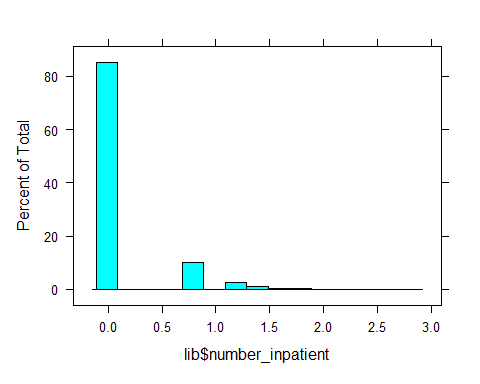
\includegraphics{Final_project_files/figure-latex/unnamed-chunk-3-1.pdf}

\begin{Shaded}
\begin{Highlighting}[]
\FunctionTok{histogram}\NormalTok{(lib}\SpecialCharTok{$}\NormalTok{number\_outpatient)}
\end{Highlighting}
\end{Shaded}

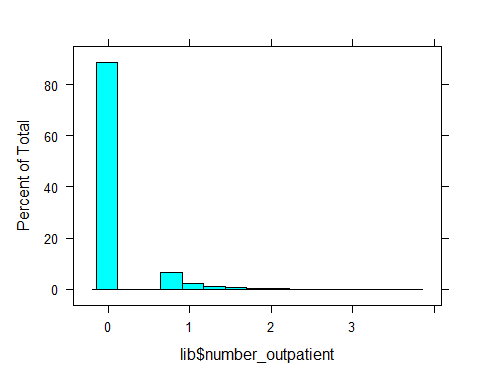
\includegraphics{Final_project_files/figure-latex/unnamed-chunk-3-2.pdf}

\begin{Shaded}
\begin{Highlighting}[]
\FunctionTok{histogram}\NormalTok{(lib}\SpecialCharTok{$}\NormalTok{number\_emergency)}
\end{Highlighting}
\end{Shaded}

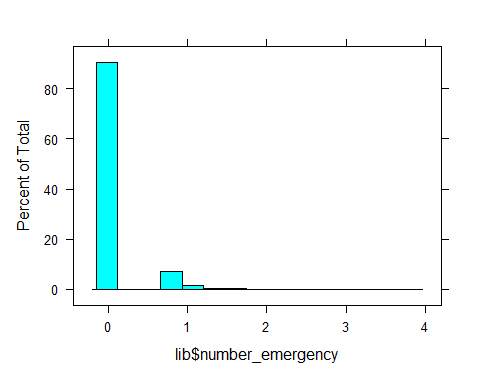
\includegraphics{Final_project_files/figure-latex/unnamed-chunk-3-3.pdf}

\begin{Shaded}
\begin{Highlighting}[]
\NormalTok{non\_outliers }\OtherTok{=} \ControlFlowTok{function}\NormalTok{(x, zs) \{}
\NormalTok{  temp }\OtherTok{\textless{}{-}}\NormalTok{ (x }\SpecialCharTok{{-}} \FunctionTok{mean}\NormalTok{(x))}\SpecialCharTok{/}\FunctionTok{sd}\NormalTok{(x)}
  \FunctionTok{return}\NormalTok{(temp }\SpecialCharTok{\textless{}}\NormalTok{ zs)}
\NormalTok{\}}



\NormalTok{lib }\OtherTok{\textless{}{-}}\NormalTok{ lib[}\FunctionTok{non\_outliers}\NormalTok{(lib}\SpecialCharTok{$}\NormalTok{number\_inpatient, }\DecValTok{3}\NormalTok{),]}
\NormalTok{lib }\OtherTok{\textless{}{-}}\NormalTok{ lib[}\FunctionTok{non\_outliers}\NormalTok{(lib}\SpecialCharTok{$}\NormalTok{number\_outpatient, }\DecValTok{3}\NormalTok{),]}
\NormalTok{lib }\OtherTok{\textless{}{-}}\NormalTok{ lib[}\FunctionTok{non\_outliers}\NormalTok{(lib}\SpecialCharTok{$}\NormalTok{number\_emergency, }\DecValTok{3}\NormalTok{),]}
\NormalTok{lib }\OtherTok{\textless{}{-}} \FunctionTok{subset}\NormalTok{(lib, }\AttributeTok{select =} \SpecialCharTok{{-}}\FunctionTok{c}\NormalTok{(number\_emergency))}



\CommentTok{\#Normalise skewed features and removing outliers using z{-}score}

\NormalTok{cols }\OtherTok{\textless{}{-}}\NormalTok{ dplyr}\SpecialCharTok{::}\FunctionTok{select\_if}\NormalTok{(lib, is.numeric)}
\NormalTok{temp }\OtherTok{\textless{}{-}} \FunctionTok{scale}\NormalTok{(dplyr}\SpecialCharTok{::}\FunctionTok{select\_if}\NormalTok{(lib, is.numeric))}
\ControlFlowTok{for}\NormalTok{(col }\ControlFlowTok{in} \FunctionTok{colnames}\NormalTok{(cols))\{}
\NormalTok{  lib[,col] }\OtherTok{\textless{}{-}}\NormalTok{ temp[,col]}
\NormalTok{\}}
\FunctionTok{str}\NormalTok{(lib)}
\end{Highlighting}
\end{Shaded}

\begin{verbatim}
## 'data.frame':    17547 obs. of  48 variables:
##  $ encounter_id              : num  -1.34 -1.33 -1.33 -1.32 -1.23 ...
##  $ patient_nbr               : num  -0.945 -0.938 -0.938 -0.934 -1.286 ...
##  $ race                      : chr  "Caucasian" "Caucasian" "Caucasian" "Caucasian" ...
##  $ gender                    : chr  "Female" "Female" "Female" "Male" ...
##  $ age                       : chr  "70" "60" "90" "70" ...
##  $ admission_type_id         : num  -1.1297 0.0569 -1.1297 -1.1297 -1.1297 ...
##  $ admission_type_name       : chr  "Emergency" "Urgent" "Emergency" "Emergency" ...
##  $ discharge_disposition_id  : num  4.4708 -0.4262 -0.4262 -0.193 0.0402 ...
##  $ discharge_disposition_name: chr  "Discharged/transferred to another rehab fac including rehab units of a hospital ." "Discharged to home" "Discharged to home" "Discharged/transferred to another short term hospital" ...
##  $ admission_source_id       : num  0.91 -1.184 0.91 0.91 0.561 ...
##  $ admission_source_name     : chr  " Emergency Room" " Physician Referral" " Emergency Room" " Emergency Room" ...
##  $ time_in_hospital          : num  0.9463 -0.4169 -0.0761 1.9687 2.6503 ...
##  $ payer_code                : chr  "MC" "MC" "MC" "MC" ...
##  $ medical_specialty         : chr  "Orthopedics-Reconstructive" "Nephrology" "Emergency/Trauma" "InternalMedicine" ...
##  $ num_lab_procedures        : num  0.849 0.899 0.748 1.354 1.808 ...
##  $ num_procedures            : num  0.238 0.79 -0.313 -0.313 1.894 ...
##  $ num_medications           : num  -0.11 -0.557 -0.781 0.226 0.338 ...
##  $ number_outpatient         : num  -0.296 -0.296 -0.296 -0.296 -0.296 ...
##  $ number_inpatient          : num  -0.365 -0.365 -0.365 -0.365 -0.365 ...
##  $ diag_1                    : chr  "821" "V56" "532" "682" ...
##  $ diag_2                    : chr  "276" "403" "428" "427" ...
##  $ diag_3                    : chr  "285" "599" "535" "276" ...
##  $ number_diagnoses          : num  0.96 -0.58 -0.58 -0.58 -1.09 ...
##  $ max_glu_serum             : chr  "0" "0" "0" "0" ...
##  $ A1Cresult                 : chr  "0" "0" "0" "0" ...
##  $ metformin                 : chr  "0" "0" "0" "1" ...
##  $ repaglinide               : chr  "0" "0" "0" "0" ...
##  $ nateglinide               : chr  "0" "0" "0" "0" ...
##  $ chlorpropamide            : chr  "0" "0" "0" "0" ...
##  $ glimepiride               : chr  "0" "0" "1" "0" ...
##  $ glipizide                 : chr  "No" "No" "No" "No" ...
##  $ glyburide                 : chr  "0" "0" "0" "0" ...
##  $ pioglitazone              : chr  "2" "0" "0" "0" ...
##  $ rosiglitazone             : chr  "No" "No" "No" "No" ...
##  $ acarbose                  : chr  "0" "0" "0" "0" ...
##  $ miglitol                  : chr  "No" "No" "No" "No" ...
##  $ tolazamide                : chr  "No" "No" "No" "No" ...
##  $ insulin                   : chr  "1" "1" "0" "1" ...
##  $ glyburide.metformin       : chr  "No" "No" "No" "No" ...
##  $ glipizide.metformin       : chr  "0" "0" "0" "0" ...
##  $ metformin.pioglitazone    : chr  "No" "No" "No" "No" ...
##  $ change                    : chr  "1" "0" "0" "1" ...
##  $ diabetesMed               : chr  "1" "1" "1" "1" ...
##  $ diagnosis                 : chr  "Injury" "Other" "Digestive" "Circulatory" ...
##  $ visits                    : num  -0.484 -0.484 -0.484 -0.484 -0.484 ...
##  $ readmitted                : chr  "NO" "NO" "NO" "NO" ...
##  $ num_med                   : num  -0.19 -0.19 -0.19 -0.19 -0.19 ...
##  $ num_changes               : num  -0.189 -0.189 -0.189 -0.189 -0.189 ...
\end{verbatim}

\begin{Shaded}
\begin{Highlighting}[]
\CommentTok{\# see c}
 \CommentTok{\# see c}
\FunctionTok{library}\NormalTok{(dplyr)}
\CommentTok{\# see c}
\FunctionTok{library}\NormalTok{(GGally)}
\end{Highlighting}
\end{Shaded}

\begin{verbatim}
## Registered S3 method overwritten by 'GGally':
##   method from   
##   +.gg   ggplot2
\end{verbatim}

\begin{Shaded}
\begin{Highlighting}[]
\FunctionTok{ggpairs}\NormalTok{(lib, }\AttributeTok{columns =} \FunctionTok{c}\NormalTok{(}\StringTok{"number\_inpatient"}\NormalTok{,}\StringTok{"num\_lab\_procedures"}\NormalTok{,}\StringTok{"number\_outpatient"}\NormalTok{,}\StringTok{"number\_diagnoses"}\NormalTok{,}
                         \StringTok{"num\_procedures"}\NormalTok{,}\StringTok{"visits"}\NormalTok{))}
\end{Highlighting}
\end{Shaded}

\includegraphics{Final_project_files/figure-latex/unnamed-chunk-4-1.pdf}

\begin{Shaded}
\begin{Highlighting}[]
\CommentTok{\# Change datatype }
\NormalTok{lib}\SpecialCharTok{$}\NormalTok{num\_med   }\OtherTok{\textless{}{-}} \FunctionTok{as.numeric}\NormalTok{(lib}\SpecialCharTok{$}\NormalTok{num\_med)}
\CommentTok{\# Change data type }
\NormalTok{lib}\SpecialCharTok{$}\NormalTok{num\_changes }\OtherTok{\textless{}{-}} \FunctionTok{as.numeric}\NormalTok{(lib}\SpecialCharTok{$}\NormalTok{num\_changes)}

\CommentTok{\# PLot all the variables }

\NormalTok{cor }\OtherTok{\textless{}{-}}\NormalTok{  lib }\SpecialCharTok{\%\textgreater{}\%}\NormalTok{ dplyr}\SpecialCharTok{::}\FunctionTok{select}\NormalTok{(number\_outpatient,number\_inpatient,visits, num\_med, num\_changes)}
\FunctionTok{plot}\NormalTok{(cor)}
\end{Highlighting}
\end{Shaded}

\includegraphics{Final_project_files/figure-latex/unnamed-chunk-4-2.pdf}

\begin{Shaded}
\begin{Highlighting}[]
\FunctionTok{library}\NormalTok{(psych)}
\end{Highlighting}
\end{Shaded}

\begin{verbatim}
## 
## Attaching package: 'psych'
\end{verbatim}

\begin{verbatim}
## The following objects are masked from 'package:ggplot2':
## 
##     %+%, alpha
\end{verbatim}

\begin{Shaded}
\begin{Highlighting}[]
\FunctionTok{corPlot}\NormalTok{(cor)}
\end{Highlighting}
\end{Shaded}

\includegraphics{Final_project_files/figure-latex/unnamed-chunk-4-3.pdf}

\begin{Shaded}
\begin{Highlighting}[]
\CommentTok{\# Model development }

\CommentTok{\# Model development }

\CommentTok{\# set seed }
\FunctionTok{set.seed}\NormalTok{(}\DecValTok{123}\NormalTok{)}
\CommentTok{\# turn row into 2 category 1 for readmitted and 0 not readmitted in the prediod of 30 days}
\NormalTok{lib}\SpecialCharTok{$}\NormalTok{readmitted }\OtherTok{\textless{}{-}} \FunctionTok{case\_when}\NormalTok{(lib}\SpecialCharTok{$}\NormalTok{readmitted }\SpecialCharTok{\%in\%} \FunctionTok{c}\NormalTok{(}\StringTok{"\textgreater{}30"}\NormalTok{,}\StringTok{"NO"}\NormalTok{) }\SpecialCharTok{\textasciitilde{}} \StringTok{"0"}\NormalTok{,}
                              \ConstantTok{TRUE} \SpecialCharTok{\textasciitilde{}} \StringTok{"1"}\NormalTok{)}

\CommentTok{\# creating  training and test }
\NormalTok{train\_indices }\OtherTok{\textless{}{-}} \FunctionTok{sample}\NormalTok{(}\FunctionTok{seq\_len}\NormalTok{(}\FunctionTok{nrow}\NormalTok{(lib)), }\FloatTok{0.7}\SpecialCharTok{*} \FunctionTok{nrow}\NormalTok{(lib))}
\NormalTok{train\_data }\OtherTok{\textless{}{-}}\NormalTok{ lib[train\_indices, ]}
\NormalTok{test\_data }\OtherTok{\textless{}{-}}\NormalTok{ lib[}\SpecialCharTok{{-}}\NormalTok{train\_indices, ]}

\CommentTok{\# Fit the logistic regression }
\NormalTok{model }\OtherTok{\textless{}{-}} \FunctionTok{glm}\NormalTok{(readmitted }\SpecialCharTok{==} \StringTok{\textquotesingle{}1\textquotesingle{}} \SpecialCharTok{\textasciitilde{}}\NormalTok{  visits }\SpecialCharTok{+}\NormalTok{ number\_inpatient }\SpecialCharTok{+}\NormalTok{ number\_outpatient  , }\AttributeTok{data =}\NormalTok{ train\_data)}
\FunctionTok{summary}\NormalTok{(model)   }
\end{Highlighting}
\end{Shaded}

\begin{verbatim}
## 
## Call:
## glm(formula = readmitted == "1" ~ visits + number_inpatient + 
##     number_outpatient, data = train_data)
## 
## Deviance Residuals: 
##      Min        1Q    Median        3Q       Max  
## -0.15409  -0.07546  -0.07546  -0.07546   0.94035  
## 
## Coefficients:
##                    Estimate Std. Error t value Pr(>|t|)    
## (Intercept)        0.080788   0.002454  32.924   <2e-16 ***
## visits             0.005823   0.006218   0.936   0.3490    
## number_inpatient   0.012472   0.004732   2.636   0.0084 ** 
## number_outpatient -0.006891   0.004397  -1.567   0.1171    
## ---
## Signif. codes:  0 '***' 0.001 '**' 0.01 '*' 0.05 '.' 0.1 ' ' 1
## 
## (Dispersion parameter for gaussian family taken to be 0.07393891)
## 
##     Null deviance: 911.04  on 12281  degrees of freedom
## Residual deviance: 907.82  on 12278  degrees of freedom
## AIC: 2872.1
## 
## Number of Fisher Scoring iterations: 2
\end{verbatim}

\begin{Shaded}
\begin{Highlighting}[]
\NormalTok{predicted\_probs }\OtherTok{\textless{}{-}} \FunctionTok{predict}\NormalTok{(model, }\AttributeTok{newdata =}\NormalTok{ test\_data , }\AttributeTok{type =} \StringTok{"response"}\NormalTok{)}

\CommentTok{\# Convert probabilities to binary predictions}
\NormalTok{predicted\_classes }\OtherTok{\textless{}{-}} \FunctionTok{ifelse}\NormalTok{(predicted\_probs }\SpecialCharTok{\textgreater{}} \FloatTok{0.1}\NormalTok{, }\StringTok{"readmitted"}\NormalTok{, }\StringTok{"Not readmitted"}\NormalTok{)}
\CommentTok{\# Convert probabilities to predicted classes}
\DocumentationTok{\#\#predicted\_classes \textless{}{-} ifelse(predicted\_probs \textgreater{} 0.5, "\textless{}30", ifelse(predicted\_probs \textgreater{} 0.25, "NO", "\textgreater{}30"))}


\CommentTok{\# Display the confusion matrix}
\NormalTok{confusion\_matrix }\OtherTok{\textless{}{-}} \FunctionTok{table}\NormalTok{(predicted\_classes, test\_data}\SpecialCharTok{$}\NormalTok{readmitted)}
\FunctionTok{print}\NormalTok{(confusion\_matrix)}
\end{Highlighting}
\end{Shaded}

\begin{verbatim}
##                  
## predicted_classes    0    1
##    Not readmitted 4261  327
##    readmitted      594   83
\end{verbatim}

\begin{Shaded}
\begin{Highlighting}[]
\CommentTok{\# Calculate accuracy}
\NormalTok{accuracy }\OtherTok{\textless{}{-}} \FunctionTok{sum}\NormalTok{(}\FunctionTok{diag}\NormalTok{(confusion\_matrix)) }\SpecialCharTok{/} \FunctionTok{sum}\NormalTok{(confusion\_matrix)}
\FunctionTok{print}\NormalTok{(}\FunctionTok{paste}\NormalTok{(}\StringTok{"Accuracy:"}\NormalTok{, accuracy))}
\end{Highlighting}
\end{Shaded}

\begin{verbatim}
## [1] "Accuracy: 0.825071225071225"
\end{verbatim}

\begin{Shaded}
\begin{Highlighting}[]
\CommentTok{\#Display the predicted labels}

\NormalTok{pred\_model\_1 }\OtherTok{\textless{}{-}}\NormalTok{ test\_data}
\NormalTok{pred\_model\_1}\SpecialCharTok{$}\NormalTok{predictor }\OtherTok{\textless{}{-}}\NormalTok{ predicted\_classes}
\FunctionTok{head}\NormalTok{(pred\_model\_1)}
\end{Highlighting}
\end{Shaded}

\begin{verbatim}
##       encounter_id patient_nbr             race gender age admission_type_id
## 24070    -1.219663   -1.100618        Caucasian Female  30       -1.12965500
## 24138    -1.217350   -1.101954        Caucasian Female  70       -1.12965500
## 24277    -1.212543   -1.180311        Caucasian Female  80       -1.12965500
## 24302    -1.211674   -1.144384        Caucasian   Male  30        0.05693921
## 24315    -1.211539   -1.066458 African American Female  80       -1.12965500
## 24345    -1.210605   -1.447905        Caucasian Female  70        0.05693921
##       admission_type_name discharge_disposition_id discharge_disposition_name
## 24070           Emergency               -0.4262194         Discharged to home
## 24138           Emergency               -0.4262194         Discharged to home
## 24277           Emergency               -0.4262194         Discharged to home
## 24302              Urgent                0.9729211                   Left AMA
## 24315           Emergency               -0.4262194         Discharged to home
## 24345              Urgent               -0.4262194         Discharged to home
##       admission_source_id                       admission_source_name
## 24070           0.5614243  Transfer from another health care facility
## 24138           0.9104398                              Emergency Room
## 24277           0.5614243  Transfer from another health care facility
## 24302          -1.1836534                          Physician Referral
## 24315           0.5614243  Transfer from another health care facility
## 24345          -1.1836534                          Physician Referral
##       time_in_hospital payer_code medical_specialty num_lab_procedures
## 24070       2.99114428         MC        Nephrology          1.7071424
## 24138      -0.75775474         MC  InternalMedicine          0.4955452
## 24277      -0.07613673         MC  InternalMedicine          0.1421626
## 24302      -0.75775474         UN  InternalMedicine          0.3440955
## 24315       0.26467227         UN  InternalMedicine          1.2023102
## 24345      -0.75775474         MC  InternalMedicine         -0.9179850
##       num_procedures num_medications number_outpatient number_inpatient diag_1
## 24070      0.2383056     0.002104749         -0.295955       -0.3652328    112
## 24138     -0.8652964    -1.005132450         -0.295955       -0.3652328    577
## 24277     -0.8652964    -0.557471472         -0.295955       -0.3652328    414
## 24302     -0.8652964    -1.117047694         -0.295955       -0.3652328    486
## 24315     -0.8652964    -1.005132450         -0.295955       -0.3652328    435
## 24345     -0.8652964    -0.781301961         -0.295955       -0.3652328    428
##       diag_2 diag_3 number_diagnoses max_glu_serum A1Cresult metformin
## 24070    996  25013        -1.093696             0         8         0
## 24138    428    414        -1.093696             0         0         0
## 24277    427    424        -1.093696             0         0         0
## 24302    493  25013        -1.093696             0         0         0
## 24315    427  25092        -1.093696             0         0         1
## 24345    250    414        -1.093696             0         0         0
##       repaglinide nateglinide chlorpropamide glimepiride glipizide glyburide
## 24070           0           0              0           0        No         0
## 24138           0           0              0           0        No         0
## 24277           0           0              0           1        No         0
## 24302           0           0              0           0        No         0
## 24315           0           0              0           0    Steady         0
## 24345           0           0              0           0        No         0
##       pioglitazone rosiglitazone acarbose miglitol tolazamide insulin
## 24070            0            No        0       No         No       1
## 24138            0            No        0       No         No       0
## 24277            0            No        0       No         No       1
## 24302            0            No        0       No         No       0
## 24315            0            No        0       No         No       0
## 24345            0            No        0       No         No       1
##       glyburide.metformin glipizide.metformin metformin.pioglitazone change
## 24070                  No                   0                     No      0
## 24138                  No                   0                     No      0
## 24277                  No                   0                     No      1
## 24302                  No                   0                     No      0
## 24315                  No                   0                     No      1
## 24345                  No                   0                     No      0
##       diabetesMed   diagnosis     visits readmitted    num_med num_changes
## 24070           1 Circulatory -0.4838539          0 -0.1898372  -0.1885303
## 24138           0   Digestive -0.4838539          0 -0.1898372  -0.1885303
## 24277           1 Circulatory -0.4838539          0 -0.1898372  -0.1885303
## 24302           0 Respiratory -0.4838539          0 -0.1898372  -0.1885303
## 24315           1 Circulatory -0.4838539          0 -0.1898372  -0.1885303
## 24345           1 Circulatory -0.4838539          0 -0.1898372  -0.1885303
##            predictor
## 24070 Not readmitted
## 24138 Not readmitted
## 24277 Not readmitted
## 24302 Not readmitted
## 24315 Not readmitted
## 24345 Not readmitted
\end{verbatim}

\begin{Shaded}
\begin{Highlighting}[]
\CommentTok{\#evaluation }
\DocumentationTok{\#\#3 second model }
\FunctionTok{library}\NormalTok{(boot)}
\end{Highlighting}
\end{Shaded}

\begin{verbatim}
## 
## Attaching package: 'boot'
\end{verbatim}

\begin{verbatim}
## The following object is masked from 'package:psych':
## 
##     logit
\end{verbatim}

\begin{verbatim}
## The following object is masked from 'package:lattice':
## 
##     melanoma
\end{verbatim}

\begin{Shaded}
\begin{Highlighting}[]
\CommentTok{\# Define the logistic regression model}
\FunctionTok{set.seed}\NormalTok{(}\DecValTok{123}\NormalTok{)}
\NormalTok{logistic\_model }\OtherTok{\textless{}{-}} \FunctionTok{glm}\NormalTok{(readmitted }\SpecialCharTok{==} \StringTok{"1"} \SpecialCharTok{\textasciitilde{}}\NormalTok{ visits }\SpecialCharTok{+}\NormalTok{ number\_outpatient  , }\AttributeTok{data =}\NormalTok{ lib)}
\FunctionTok{summary}\NormalTok{(logistic\_model)}
\end{Highlighting}
\end{Shaded}

\begin{verbatim}
## 
## Call:
## glm(formula = readmitted == "1" ~ visits + number_outpatient, 
##     data = lib)
## 
## Deviance Residuals: 
##      Min        1Q    Median        3Q       Max  
## -0.16832  -0.07363  -0.07363  -0.07363   0.93571  
## 
## Coefficients:
##                    Estimate Std. Error t value Pr(>|t|)    
## (Intercept)        0.079843   0.002043  39.083  < 2e-16 ***
## visits             0.021064   0.002723   7.735 1.09e-14 ***
## number_outpatient -0.013437   0.002723  -4.934 8.14e-07 ***
## ---
## Signif. codes:  0 '***' 0.001 '**' 0.01 '*' 0.05 '.' 0.1 ' ' 1
## 
## (Dispersion parameter for gaussian family taken to be 0.07323046)
## 
##     Null deviance: 1289.1  on 17546  degrees of freedom
## Residual deviance: 1284.8  on 17544  degrees of freedom
## AIC: 3930.8
## 
## Number of Fisher Scoring iterations: 2
\end{verbatim}

\begin{Shaded}
\begin{Highlighting}[]
\CommentTok{\# Perform 10{-}fold cross{-}validation}
\NormalTok{cv\_results }\OtherTok{\textless{}{-}} \FunctionTok{cv.glm}\NormalTok{(lib, logistic\_model, }\AttributeTok{K =} \DecValTok{10}\NormalTok{)}

\DocumentationTok{\#\#print(cv\_results)}

\CommentTok{\# Access accuracy}
\NormalTok{accuracy2 }\OtherTok{\textless{}{-}} \DecValTok{1} \SpecialCharTok{{-}}\NormalTok{ cv\_results}\SpecialCharTok{$}\NormalTok{delta[}\DecValTok{1}\NormalTok{]}
\FunctionTok{cat}\NormalTok{(}\StringTok{"Accuracy:"}\NormalTok{, accuracy2, }\StringTok{"}\SpecialCharTok{\textbackslash{}n}\StringTok{"}\NormalTok{)}
\end{Highlighting}
\end{Shaded}

\begin{verbatim}
## Accuracy: 0.9267509
\end{verbatim}

\begin{Shaded}
\begin{Highlighting}[]
\CommentTok{\# Predict the probabilities of the positive class ("Wins")}
\NormalTok{predicted\_probs2 }\OtherTok{\textless{}{-}} \FunctionTok{predict}\NormalTok{(logistic\_model, }\AttributeTok{newdata =}\NormalTok{ lib, }\AttributeTok{type =} \StringTok{"response"}\NormalTok{)}


\CommentTok{\# Convert probabilities to binary predictions}
\NormalTok{predicted\_labels2 }\OtherTok{\textless{}{-}}\NormalTok{ predicted\_classes }\OtherTok{\textless{}{-}} \FunctionTok{ifelse}\NormalTok{(predicted\_probs2 }\SpecialCharTok{\textgreater{}} \FloatTok{0.1}\NormalTok{, }\StringTok{"readmitted"}\NormalTok{, }\StringTok{"Not readmitted"}\NormalTok{)}

\CommentTok{\# Display results}
\CommentTok{\#print(data.frame(Probabilities = predicted\_probs2, Predicted\_Labels = predicted\_labels2))}
\NormalTok{at2 }\OtherTok{\textless{}{-}} \FunctionTok{data.frame}\NormalTok{(}\AttributeTok{Probabilities =}\NormalTok{ predicted\_probs2, }\AttributeTok{Predicted\_Labels =}\NormalTok{ predicted\_labels2)}
\FunctionTok{head}\NormalTok{(at2)}
\end{Highlighting}
\end{Shaded}

\begin{verbatim}
##       Probabilities Predicted_Labels
## 20447    0.07362731   Not readmitted
## 20738    0.07362731   Not readmitted
## 20825    0.07362731   Not readmitted
## 21084    0.07362731   Not readmitted
## 23880    0.07362731   Not readmitted
## 23923    0.07362731   Not readmitted
\end{verbatim}

\begin{Shaded}
\begin{Highlighting}[]
\CommentTok{\# Display the confusion matrix}
\NormalTok{confusion\_matrix2 }\OtherTok{\textless{}{-}} \FunctionTok{table}\NormalTok{(predicted\_labels2, lib}\SpecialCharTok{$}\NormalTok{readmitted)}
\FunctionTok{print}\NormalTok{(confusion\_matrix2)}
\end{Highlighting}
\end{Shaded}

\begin{verbatim}
##                  
## predicted_labels2     0     1
##    Not readmitted 13617  1087
##    readmitted      2529   314
\end{verbatim}

\begin{Shaded}
\begin{Highlighting}[]
\CommentTok{\# Display the predicted labels}
\CommentTok{\#print(predicted\_labels2)}
\NormalTok{pred\_model2 }\OtherTok{\textless{}{-}}\NormalTok{ lib}
\NormalTok{pred\_model2}\SpecialCharTok{$}\NormalTok{predictor }\OtherTok{\textless{}{-}}\NormalTok{ predicted\_labels2}
\FunctionTok{head}\NormalTok{(pred\_model2)}
\end{Highlighting}
\end{Shaded}

\begin{verbatim}
##       encounter_id patient_nbr      race gender age admission_type_id
## 20447    -1.338575  -0.9452118 Caucasian Female  70       -1.12965500
## 20738    -1.329333  -0.9384905 Caucasian Female  60        0.05693921
## 20825    -1.326727  -0.9376905 Caucasian Female  90       -1.12965500
## 21084    -1.318555  -0.9341307 Caucasian   Male  70       -1.12965500
## 23880    -1.225515  -1.2857602 Caucasian Female  70       -1.12965500
## 23923    -1.224257  -1.0683153 Caucasian   Male  70       -1.12965500
##       admission_type_name discharge_disposition_id
## 20447           Emergency               4.47077231
## 20738              Urgent              -0.42621943
## 20825           Emergency              -0.42621943
## 21084           Emergency              -0.19302935
## 23880           Emergency               0.04016074
## 23923           Emergency               0.04016074
##                                                              discharge_disposition_name
## 20447 Discharged/transferred to another rehab fac including rehab units of a hospital .
## 20738                                                                Discharged to home
## 20825                                                                Discharged to home
## 21084                             Discharged/transferred to another short term hospital
## 23880                                                     Discharged/transferred to SNF
## 23923                                                     Discharged/transferred to SNF
##       admission_source_id                       admission_source_name
## 20447           0.9104398                              Emergency Room
## 20738          -1.1836534                          Physician Referral
## 20825           0.9104398                              Emergency Room
## 21084           0.9104398                              Emergency Room
## 23880           0.5614243  Transfer from another health care facility
## 23923           0.5614243  Transfer from another health care facility
##       time_in_hospital payer_code          medical_specialty num_lab_procedures
## 20447       0.94629027         MC Orthopedics-Reconstructive          0.8489277
## 20738      -0.41694574         MC                 Nephrology          0.8994109
## 20825      -0.07613673         MC           Emergency/Trauma          0.7479613
## 21084       1.96871727         MC           InternalMedicine          1.3537599
## 23880       2.65033527         UN           InternalMedicine          1.8081089
## 23923       2.65033527         MC           InternalMedicine          0.9498941
##       num_procedures num_medications number_outpatient number_inpatient diag_1
## 20447      0.2383056      -0.1098105         -0.295955       -0.3652328    821
## 20738      0.7901065      -0.5574715         -0.295955       -0.3652328    V56
## 20825     -0.3134954      -0.7813020         -0.295955       -0.3652328    532
## 21084     -0.3134954       0.2259352         -0.295955       -0.3652328    682
## 23880      1.8937085       0.3378505         -0.295955       -0.3652328    238
## 23923      1.8937085      -0.6693867         -0.295955       -0.3652328    532
##       diag_2 diag_3 number_diagnoses max_glu_serum A1Cresult metformin
## 20447    276    285        0.9603645             0         0         0
## 20738    403    599       -0.5801812             0         0         0
## 20825    428    535       -0.5801812             0         0         0
## 21084    427    276       -0.5801812             0         0         1
## 23880  25002    733       -1.0936964             0         8         0
## 23923    280    569       -1.0936964             0         0         0
##       repaglinide nateglinide chlorpropamide glimepiride glipizide glyburide
## 20447           0           0              0           0        No         0
## 20738           0           0              0           0        No         0
## 20825           0           0              0           1        No         0
## 21084           0           0              0           0        No         0
## 23880           0           0              0           0        No         0
## 23923           0           0              0           0        No         0
##       pioglitazone rosiglitazone acarbose miglitol tolazamide insulin
## 20447            2            No        0       No         No       1
## 20738            0            No        0       No         No       1
## 20825            0            No        0       No         No       0
## 21084            0            No        0       No         No       1
## 23880            0            No        0       No         No       1
## 23923            0            No        0       No         No       0
##       glyburide.metformin glipizide.metformin metformin.pioglitazone change
## 20447                  No                   0                     No      1
## 20738                  No                   0                     No      0
## 20825                  No                   0                     No      0
## 21084                  No                   0                     No      1
## 23880                  No                   0                     No      0
## 23923                  No                   0                     No      0
##       diabetesMed   diagnosis     visits readmitted    num_med num_changes
## 20447           1      Injury -0.4838539          0 -0.1898372  -0.1885303
## 20738           1       Other -0.4838539          0 -0.1898372  -0.1885303
## 20825           1   Digestive -0.4838539          0 -0.1898372  -0.1885303
## 21084           1 Circulatory -0.4838539          0 -0.1898372  -0.1885303
## 23880           1   Neoplasms -0.4838539          0 -0.1898372  -0.1885303
## 23923           0   Digestive -0.4838539          0 -0.1898372  -0.1885303
##            predictor
## 20447 Not readmitted
## 20738 Not readmitted
## 20825 Not readmitted
## 21084 Not readmitted
## 23880 Not readmitted
## 23923 Not readmitted
\end{verbatim}

\hypertarget{model-evaluations}{%
\subsubsection{Model Evaluations}\label{model-evaluations}}

We create a multiple regression model with an accuracy 0.82 with the
encoded data set. we split the data into train and test set. We notice
that there are steps we can do improve the model accuracy. We add more
predictors to the second model and implement a cross validation of 10
folds. We were able to achieve an accuracy of 0.92. we try to add more
categorical features to the multiple regression and use cross validation
of 10 folds to improve the model accuracy to 0.802. We use logistic
regression to predict the categorical value of readmitted against the
most correlated predictors. we achieved an accuracy of 0.627.

the second model will be selected to predict the readmission data. There
are still a lot of work to get done specially in data reprocessing. We
manage to achieve a high accuracy but QQ plots for every model show data
are not well distributed.

\hypertarget{limitation}{%
\subsection{Limitation}\label{limitation}}

There are still outliers in the data set even we used standard deviation
to be removed. Data collected should contains more relevant columns that
related that are related to diabetes.

\begin{Shaded}
\begin{Highlighting}[]
\DocumentationTok{\#\#\#\#\#\#\#\#\#\#\#\#\#\#\#\#\#\#\#\#\#\#\#\#\#\#\#\#\#\#\#\#\#\#\#\#\#\#\#\#\#\#\#\#\#\#\#\#\#\#\#\#\#}
\CommentTok{\# create a new model logistic model with other predictors }
\FunctionTok{set.seed}\NormalTok{(}\DecValTok{123}\NormalTok{)}
\NormalTok{logistic\_model2 }\OtherTok{\textless{}{-}}\FunctionTok{glm}\NormalTok{(readmitted}\SpecialCharTok{==} \StringTok{"1"}  \SpecialCharTok{\textasciitilde{}}\NormalTok{ age }\SpecialCharTok{+}\NormalTok{ visits }\SpecialCharTok{+}\NormalTok{ number\_outpatient }\SpecialCharTok{+}\NormalTok{ max\_glu\_serum }\SpecialCharTok{+}\NormalTok{ insulin }\SpecialCharTok{+}\NormalTok{ diabetesMed , }\AttributeTok{data =}\NormalTok{ lib)}
\FunctionTok{summary}\NormalTok{(logistic\_model2)}
\end{Highlighting}
\end{Shaded}

\begin{verbatim}
## 
## Call:
## glm(formula = readmitted == "1" ~ age + visits + number_outpatient + 
##     max_glu_serum + insulin + diabetesMed, data = lib)
## 
## Deviance Residuals: 
##      Min        1Q    Median        3Q       Max  
## -0.19364  -0.09269  -0.07753  -0.05726   0.99242  
## 
## Coefficients:
##                    Estimate Std. Error t value Pr(>|t|)    
## (Intercept)       -0.008688   0.155913  -0.056  0.95556    
## age10             -0.006254   0.160276  -0.039  0.96888    
## age20              0.039639   0.156814   0.253  0.80045    
## age30              0.043047   0.156301   0.275  0.78301    
## age40              0.042740   0.156063   0.274  0.78419    
## age50              0.047020   0.155999   0.301  0.76311    
## age60              0.063696   0.155982   0.408  0.68302    
## age70              0.072645   0.155974   0.466  0.64140    
## age80              0.078862   0.156000   0.506  0.61320    
## age90              0.084925   0.156375   0.543  0.58708    
## visits             0.020053   0.002722   7.367 1.82e-13 ***
## number_outpatient -0.012827   0.002724  -4.710 2.50e-06 ***
## max_glu_serum100  -0.082886   0.191010  -0.434  0.66434    
## insulin1           0.003591   0.005739   0.626  0.53147    
## insulin2           0.014393   0.007116   2.023  0.04312 *  
## insulin3           0.018947   0.007150   2.650  0.00806 ** 
## diabetesMed1       0.024835   0.006368   3.900 9.67e-05 ***
## ---
## Signif. codes:  0 '***' 0.001 '**' 0.01 '*' 0.05 '.' 0.1 ' ' 1
## 
## (Dispersion parameter for gaussian family taken to be 0.07290601)
## 
##     Null deviance: 1289.1  on 17546  degrees of freedom
## Residual deviance: 1278.0  on 17530  degrees of freedom
## AIC: 3866.9
## 
## Number of Fisher Scoring iterations: 2
\end{verbatim}

\begin{Shaded}
\begin{Highlighting}[]
\CommentTok{\# Perform 10{-}fold cross{-}validation}
\NormalTok{cv\_results2 }\OtherTok{\textless{}{-}} \FunctionTok{cv.glm}\NormalTok{(lib, logistic\_model2, }\AttributeTok{K =} \DecValTok{10}\NormalTok{)}

\FunctionTok{head}\NormalTok{(cv\_results2)}
\end{Highlighting}
\end{Shaded}

\begin{verbatim}
## $call
## cv.glm(data = lib, glmfit = logistic_model2, K = 10)
## 
## $K
## [1] 10
## 
## $delta
## [1] 0.07296679 0.07295988
## 
## $seed
##   [1]       10403         624  -983674937   643431772  1162448557  -959247990
##   [7]  -133913213  2107846888   370274761 -2022780170  -412390145   848182068
##  [13]  -266662747 -1309507294  1356997179  1661823040  1749531457  -516669426
##  [19]  1042678071 -1279933428  -410084963  1151007674  -895613453  1288379032
##  [25]  -376044615 -1358274522   307686511   101447652  1796216213 -1567696558
##  [31]  1186934955 -1925339152  -472470735    80319294 -1524429145   326645436
##  [37]  -389586803  -400786966  -890731933  -852332472  1365217705 -1785317034
##  [43] -1551153185  1359863956  2098748037 -1013039742  -329721061 -1587358816
##  [49]   344102689 -1520389522   166492183  1821136236  1646453629  1056605210
##  [55] -1419044141  -806080008   520985497   711286406  2004844367 -1445006012
##  [61]  1329781621 -1188844110 -1089068661  1173875536 -1983217903   514629022
##  [67]  -237421177  -258138084  -930078099   261626442  1349308227 -1125425240
##  [73] -1677778551    25874358   409637567 -1987430924  1583257701  -136173086
##  [79]   639501307   272101120 -1024630015 -1994369842  -939499785 -1944742196
##  [85]  -591520419 -1994900358  1072996275  1119025496  2035491705 -2082894618
##  [91]   776176175   -69557596  1794806101  -178474478  -497581461   874372784
##  [97]   518669041  -370223106  1295572071 -1776240260 -1692674995  1935534762
## [103]   298421283   111542024 -1075273367   518297110  -289321569  1331379028
## [109]  1768277573  1473660482  2120850651   879016544  -864018719  1661675310
## [115]   135902679 -2136373204   735594301  1594631386  -546138989  1423929528
## [121] -1067541671  1962863430 -1923418865  -984154108  1907308341   642901618
## [127] -1095019701 -1836613104 -1171392815  1663582814 -1258689721 -2007301412
## [133]  -756910547  -712643830 -1271482109  -801485208    51646793 -1925477258
## [139] -1421379457  1104736436 -1348082651  -124611934   292791739  2126591424
## [145] -2043491647  -709285490 -1242530633  1688217996  -538353379 -1997652678
## [151]   -48432781   575772696   942146361    57506214  -948054033   -72610460
## [157]  1389939989   656100050   -25586645 -2012424848  1854773937  1391516862
## [163] -2100008409  -140248004 -1638135795 -2077746326  -118729245 -1417654840
## [169]   662270249   942125782 -1363864737   744183316  2123821573   -80802046
## [175] -1753997669  1277518112  1090348705  1338137582   423408535   -28214548
## [181]  1164536573  1524008346   673959507   853634936 -1599644903 -2135083002
## [187]  -345756977 -1070478652   971985653  -556736718  -406174453   663083216
## [193]  1258368657  1306568478  1820350727 -1068259940  -402617875  1499233226
## [199] -1121819965 -1773142744  1796260105  1463879990   901914175   104491892
## [205]  1605431269 -1933329566  1688405883  -446088064  1238889089   197049934
## [211]  -709469577 -1072333748  1691378909 -1260585478   198644531  2053568216
## [217]   903127801 -1970919834  -473567825  1614821412 -1905604395  1082827666
## [223]  1558537707  1875545136  1518383729 -1265655426 -2085242905  1791098620
## [229]  1447558093 -1153758166   -99557469   -92185464 -2016280343  1847562134
## [235]  1495701791  -221368108   409722309  -429353022  1765302363  2137311200
## [241]  -373658015   273043630  -350916265  -935055956    43404989    52012634
## [247]  1867958291  1488596536 -1347953959   174081222  2002460815  1429165444
## [253]  -205312331  1264621554  -603785525  1270017936 -1543231919 -1282028578
## [259]   908887751   726075484  1269456301 -1680094070  -990917501 -1377014808
## [265] -1279971127  1281050102   228230143  1097770548 -1438663771  1295361058
## [271]   829172027   988808000  1704778305   804328206 -1257113545  -516583668
## [277] -1624037219  1034190522   904064243 -1716316776  1108935353   904106790
## [283]  1222361967  1146561252  1232110741   174767186  2136668075 -1843985680
## [289]   713263665  1133192766  1302119847  -499465796  -425742451  2035727594
## [295]  1324820835  -227988664 -1598926679   227290198   601218783  1836305300
## [301]  1386514821   306372738  -445226469   618852000   -25741791   156697966
## [307]  -345772265 -2126405524  1998516861  -392853734  1588822483  1965665528
## [313] -1658840423 -1901588090  -687876529   -15753148 -1427453323 -1799286606
## [319]   -47880053    97437264  -319365615   688369822  -272731001   469052188
## [325]    27259245  1573117258  -446761405  1976539816  2093047945   424297142
## [331]  1217440191   506831092 -1961736347 -1834464030  1234111227   907381248
## [337]  -247365119   118499278 -1581033993  -893361716 -2100188067   335855482
## [343]    83920563 -1896483752  -323673479  -498745370  2088720687 -2102342236
## [349]  1873412181   226202898 -1483060885  1437743536  -430562831  -190616834
## [355] -1639345305   281953404   857940813  -549769814  -245419229  1375189512
## [361]  -237346711   590186774    75687071   655107668   151057733   930998594
## [367] -1108466725  1398789472  1995685345  1605663278  1206398167 -1945513172
## [373]  1992513085  1544169434  1610742675  -152048712  -657450407  1247059526
## [379]  1880247311  -124605692   723920437 -1548596878  1827773003   479812880
## [385]   228152785    49698142   922100295 -1524757028  -845069011   534031882
## [391]  -131080189   213485928   636833865   718143350 -1134260353 -2024842316
## [397] -1108831451  1977333154  1053535419  1301926080  -997856831   366738574
## [403] -1450544201  1064694924 -1016336355  -390217670 -1024466829   686789400
## [409] -2056715719   745319590  -999248145 -1240647580 -1395180523 -1837290030
## [415]  -681354453  -514051984  1438153137  2090364862  -209968857  1765574460
## [421]  -544057587  -844603798 -1693909789 -1746073400 -1156960215  2076419542
## [427] -1326601633  1784103188  -683597563  -824593918  1683989915  -509903840
## [433]   183502241  -132206866  -295556457   190629356 -1790739971  1849133210
## [439] -1660799661   214755960 -1837639143   975563526  1750237647  1014527428
## [445]     3490293   552878642   220695563   382907344 -1381266031  1445050910
## [451]  1771278343 -1719553892   862869741   583941834 -1759344189  1365915688
## [457]  -820969463 -1381598154   -19516097   662427252 -1098735899  -812655006
## [463]  1658982011 -1203972224  1999245697 -1592487602 -1708699273 -1038727348
## [469]  -725486627   747602170  2037447219  -161484328   469017081  1897421158
## [475]   644859055   959210276  1824012245 -1573943662  -797561621   466937648
## [481]     6984049  1344943230 -1963692313   507873788  1336756941  -446804182
## [487]  -978024797    50927496   -66994199 -1542552938 -1630130145  1108679636
## [493]   421858501   286669506   176875355  1716904672   841747809  2002101166
## [499] -1936594857  -503678804   643784125  -270685862    -9162989 -1518294728
## [505] -1177069095   450623430 -1518307441 -2055143292  1977097653  1967586034
## [511]  2139569611   993708688   887981393  -146153762 -1521041977 -1948249252
## [517]  1992764589  1735430026   469169027  -492722456  1473540041 -1902921482
## [523]  1705351935  1769673012  -929011035   948225826  -946720709  1824431680
## [529]  1626208577 -1384520178    22671159 -1788782068  -359417955   272236986
## [535]  -230435853  1174868120 -2145910343  -855063002  1748802159   651054564
## [541]  -619908203    89300818   345161387 -1411621392   774662449 -1541883586
## [547]  1651670183   581520572 -1489764723 -2028142614 -1423847325 -1844713912
## [553]  1954615209  -389144746    66876895  2030417556  -361973627  -151813246
## [559] -1573918437   944703904   610784545  1108957294 -1875417577 -1297945748
## [565]  1037500797  1908181530   823650515  1875585016   -22111847  1765196934
## [571]  -849597105  1315720004 -1748059787  -915770446   634433419 -1869504176
## [577]  -887145199  2066662302  -939545721  -822528484 -1687437203 -1367629750
## [583] -1603461821   522180008  1610588041  2052437430   110280895  2014120948
## [589]  -670960027   159018978  1050415611   568272128 -1718509311    -3409202
## [595]   753028343 -1139331892  -123651235 -2072165766 -1222087245   648343384
## [601]  1100161401   486404838   261566511  1504901284  -476745899  1151760402
## [607]  -445050773  -130902864  -423755535  1831075326   934693479   690474876
## [613]  -907644339  -744197974  1158732323    62223624 -1538777239  1455586326
## [619]  -702514273 -1712778924   651699269   959548482  -586241317  1850142816
## [625]  -647799583  2099891502
\end{verbatim}

\begin{Shaded}
\begin{Highlighting}[]
\CommentTok{\# Access accuracy}
\NormalTok{accuracy3 }\OtherTok{\textless{}{-}} \DecValTok{1} \SpecialCharTok{{-}}\NormalTok{ cv\_results2}\SpecialCharTok{$}\NormalTok{delta[}\DecValTok{1}\NormalTok{]}
\FunctionTok{cat}\NormalTok{(}\StringTok{"Accuracy:"}\NormalTok{, accuracy3, }\StringTok{"}\SpecialCharTok{\textbackslash{}n}\StringTok{"}\NormalTok{)}
\end{Highlighting}
\end{Shaded}

\begin{verbatim}
## Accuracy: 0.9270332
\end{verbatim}

\begin{Shaded}
\begin{Highlighting}[]
\CommentTok{\# Predict the probabilities of the positive class ("Wins")}
\NormalTok{predicted\_probs3 }\OtherTok{\textless{}{-}} \FunctionTok{predict}\NormalTok{(logistic\_model2, }\AttributeTok{newdata =}\NormalTok{ lib, }\AttributeTok{type =} \StringTok{"response"}\NormalTok{)}


\CommentTok{\# Convert probabilities to binary predictions}
\NormalTok{predicted\_labels3 }\OtherTok{\textless{}{-}} \FunctionTok{ifelse}\NormalTok{(predicted\_probs3 }\SpecialCharTok{\textgreater{}} \FloatTok{0.1}\NormalTok{, }\StringTok{"readmitted"}\NormalTok{, }\StringTok{"Not readmitted"}\NormalTok{)}

\CommentTok{\# Display results}
\CommentTok{\#print(data.frame(Probabilities = predicted\_probs3, Predicted\_Labels = predicted\_labels3))}
\NormalTok{at }\OtherTok{\textless{}{-}} \FunctionTok{data.frame}\NormalTok{(}\AttributeTok{Probabilities =}\NormalTok{ predicted\_probs3, }\AttributeTok{Predicted\_Labels =}\NormalTok{ predicted\_labels3) }\SpecialCharTok{\%\textgreater{}\%} \FunctionTok{arrange}\NormalTok{(}\FunctionTok{desc}\NormalTok{(Probabilities))}
\FunctionTok{head}\NormalTok{(at)}
\end{Highlighting}
\end{Shaded}

\begin{verbatim}
##       Probabilities Predicted_Labels
## 59841     0.1936381       readmitted
## 36935     0.1919764       readmitted
## 38066     0.1919764       readmitted
## 52957     0.1919764       readmitted
## 54845     0.1919764       readmitted
## 98779     0.1919764       readmitted
\end{verbatim}

\begin{Shaded}
\begin{Highlighting}[]
\CommentTok{\# Display the predicted labels}
\CommentTok{\#print(predicted\_labels3)}
\NormalTok{pred\_model3 }\OtherTok{\textless{}{-}}\NormalTok{ lib}
\NormalTok{pred\_model3}\SpecialCharTok{$}\NormalTok{predictor }\OtherTok{\textless{}{-}}\NormalTok{ predicted\_labels3}
\FunctionTok{head}\NormalTok{(pred\_model3)}
\end{Highlighting}
\end{Shaded}

\begin{verbatim}
##       encounter_id patient_nbr      race gender age admission_type_id
## 20447    -1.338575  -0.9452118 Caucasian Female  70       -1.12965500
## 20738    -1.329333  -0.9384905 Caucasian Female  60        0.05693921
## 20825    -1.326727  -0.9376905 Caucasian Female  90       -1.12965500
## 21084    -1.318555  -0.9341307 Caucasian   Male  70       -1.12965500
## 23880    -1.225515  -1.2857602 Caucasian Female  70       -1.12965500
## 23923    -1.224257  -1.0683153 Caucasian   Male  70       -1.12965500
##       admission_type_name discharge_disposition_id
## 20447           Emergency               4.47077231
## 20738              Urgent              -0.42621943
## 20825           Emergency              -0.42621943
## 21084           Emergency              -0.19302935
## 23880           Emergency               0.04016074
## 23923           Emergency               0.04016074
##                                                              discharge_disposition_name
## 20447 Discharged/transferred to another rehab fac including rehab units of a hospital .
## 20738                                                                Discharged to home
## 20825                                                                Discharged to home
## 21084                             Discharged/transferred to another short term hospital
## 23880                                                     Discharged/transferred to SNF
## 23923                                                     Discharged/transferred to SNF
##       admission_source_id                       admission_source_name
## 20447           0.9104398                              Emergency Room
## 20738          -1.1836534                          Physician Referral
## 20825           0.9104398                              Emergency Room
## 21084           0.9104398                              Emergency Room
## 23880           0.5614243  Transfer from another health care facility
## 23923           0.5614243  Transfer from another health care facility
##       time_in_hospital payer_code          medical_specialty num_lab_procedures
## 20447       0.94629027         MC Orthopedics-Reconstructive          0.8489277
## 20738      -0.41694574         MC                 Nephrology          0.8994109
## 20825      -0.07613673         MC           Emergency/Trauma          0.7479613
## 21084       1.96871727         MC           InternalMedicine          1.3537599
## 23880       2.65033527         UN           InternalMedicine          1.8081089
## 23923       2.65033527         MC           InternalMedicine          0.9498941
##       num_procedures num_medications number_outpatient number_inpatient diag_1
## 20447      0.2383056      -0.1098105         -0.295955       -0.3652328    821
## 20738      0.7901065      -0.5574715         -0.295955       -0.3652328    V56
## 20825     -0.3134954      -0.7813020         -0.295955       -0.3652328    532
## 21084     -0.3134954       0.2259352         -0.295955       -0.3652328    682
## 23880      1.8937085       0.3378505         -0.295955       -0.3652328    238
## 23923      1.8937085      -0.6693867         -0.295955       -0.3652328    532
##       diag_2 diag_3 number_diagnoses max_glu_serum A1Cresult metformin
## 20447    276    285        0.9603645             0         0         0
## 20738    403    599       -0.5801812             0         0         0
## 20825    428    535       -0.5801812             0         0         0
## 21084    427    276       -0.5801812             0         0         1
## 23880  25002    733       -1.0936964             0         8         0
## 23923    280    569       -1.0936964             0         0         0
##       repaglinide nateglinide chlorpropamide glimepiride glipizide glyburide
## 20447           0           0              0           0        No         0
## 20738           0           0              0           0        No         0
## 20825           0           0              0           1        No         0
## 21084           0           0              0           0        No         0
## 23880           0           0              0           0        No         0
## 23923           0           0              0           0        No         0
##       pioglitazone rosiglitazone acarbose miglitol tolazamide insulin
## 20447            2            No        0       No         No       1
## 20738            0            No        0       No         No       1
## 20825            0            No        0       No         No       0
## 21084            0            No        0       No         No       1
## 23880            0            No        0       No         No       1
## 23923            0            No        0       No         No       0
##       glyburide.metformin glipizide.metformin metformin.pioglitazone change
## 20447                  No                   0                     No      1
## 20738                  No                   0                     No      0
## 20825                  No                   0                     No      0
## 21084                  No                   0                     No      1
## 23880                  No                   0                     No      0
## 23923                  No                   0                     No      0
##       diabetesMed   diagnosis     visits readmitted    num_med num_changes
## 20447           1      Injury -0.4838539          0 -0.1898372  -0.1885303
## 20738           1       Other -0.4838539          0 -0.1898372  -0.1885303
## 20825           1   Digestive -0.4838539          0 -0.1898372  -0.1885303
## 21084           1 Circulatory -0.4838539          0 -0.1898372  -0.1885303
## 23880           1   Neoplasms -0.4838539          0 -0.1898372  -0.1885303
## 23923           0   Digestive -0.4838539          0 -0.1898372  -0.1885303
##            predictor
## 20447 Not readmitted
## 20738 Not readmitted
## 20825 Not readmitted
## 21084 Not readmitted
## 23880 Not readmitted
## 23923 Not readmitted
\end{verbatim}

\begin{Shaded}
\begin{Highlighting}[]
\CommentTok{\# Display the confusion matrix}
\NormalTok{confusion\_matrix3 }\OtherTok{\textless{}{-}} \FunctionTok{table}\NormalTok{(predicted\_labels3, lib}\SpecialCharTok{$}\NormalTok{readmitted)}
\CommentTok{\#print(confusion\_matrix3)}


\CommentTok{\# linear regression }
\NormalTok{model22 }\OtherTok{\textless{}{-}} \FunctionTok{lm}\NormalTok{(}\FunctionTok{as.numeric}\NormalTok{(}\FunctionTok{as.factor}\NormalTok{(readmitted)) }\SpecialCharTok{\textasciitilde{}}\NormalTok{ visits }\SpecialCharTok{+}\NormalTok{ number\_outpatient , }\AttributeTok{data =}\NormalTok{ train\_data)}
\FunctionTok{summary}\NormalTok{(model22)}
\end{Highlighting}
\end{Shaded}

\begin{verbatim}
## 
## Call:
## lm(formula = as.numeric(as.factor(readmitted)) ~ visits + number_outpatient, 
##     data = train_data)
## 
## Residuals:
##      Min       1Q   Median       3Q      Max 
## -0.16422 -0.07548 -0.07548 -0.07548  0.93941 
## 
## Coefficients:
##                    Estimate Std. Error t value Pr(>|t|)    
## (Intercept)        1.080710   0.002454 440.350  < 2e-16 ***
## visits             0.019739   0.003285   6.008 1.93e-09 ***
## number_outpatient -0.014609   0.003282  -4.452 8.58e-06 ***
## ---
## Signif. codes:  0 '***' 0.001 '**' 0.01 '*' 0.05 '.' 0.1 ' ' 1
## 
## Residual standard error: 0.272 on 12279 degrees of freedom
## Multiple R-squared:  0.002967,   Adjusted R-squared:  0.002805 
## F-statistic: 18.27 on 2 and 12279 DF,  p-value: 1.192e-08
\end{verbatim}

\begin{Shaded}
\begin{Highlighting}[]
\CommentTok{\# Make predictions}
\NormalTok{predictions5 }\OtherTok{\textless{}{-}} \FunctionTok{predict}\NormalTok{(model22, }\AttributeTok{newdata =}\NormalTok{ test\_data)}

\NormalTok{predicted\_probs22 }\OtherTok{\textless{}{-}} \FunctionTok{predict}\NormalTok{(model22, }\AttributeTok{newdata =}\NormalTok{ test\_data , }\AttributeTok{type =} \StringTok{"response"}\NormalTok{)}

\CommentTok{\# Convert probabilities to binary predictions}
\NormalTok{predicted\_classes22 }\OtherTok{\textless{}{-}} \FunctionTok{ifelse}\NormalTok{(predicted\_probs22 }\SpecialCharTok{\textgreater{}} \FloatTok{0.1}\NormalTok{, }\StringTok{"Readmitted"}\NormalTok{, }\StringTok{"Not readmitted"}\NormalTok{)}
\CommentTok{\# Calculate RMSE}
\NormalTok{rmse }\OtherTok{\textless{}{-}} \FunctionTok{sqrt}\NormalTok{(}\FunctionTok{mean}\NormalTok{((}\FunctionTok{as.numeric}\NormalTok{(}\FunctionTok{as.factor}\NormalTok{(train\_data}\SpecialCharTok{$}\NormalTok{readmitted)) }\SpecialCharTok{{-}}\NormalTok{ predictions5)}\SpecialCharTok{\^{}}\DecValTok{2}\NormalTok{))}
\end{Highlighting}
\end{Shaded}

\begin{verbatim}
## Warning in as.numeric(as.factor(train_data$readmitted)) - predictions5: longer
## object length is not a multiple of shorter object length
\end{verbatim}

\begin{Shaded}
\begin{Highlighting}[]
\CommentTok{\# Evaluate accuracy (you might want to use a suitable metric for regression, e.g., RMSE)}
\NormalTok{accuracy5 }\OtherTok{\textless{}{-}} \FunctionTok{sqrt}\NormalTok{(}\FunctionTok{mean}\NormalTok{((}\FunctionTok{as.numeric}\NormalTok{(test\_data}\SpecialCharTok{$}\NormalTok{readmitted) }\SpecialCharTok{{-}}\NormalTok{ predictions5)}\SpecialCharTok{\^{}}\DecValTok{2}\NormalTok{))}
\NormalTok{accuracy5}
\end{Highlighting}
\end{Shaded}

\begin{verbatim}
## [1] 1.037928
\end{verbatim}

\begin{Shaded}
\begin{Highlighting}[]
\CommentTok{\# Display results}
\FunctionTok{print}\NormalTok{(}\FunctionTok{paste}\NormalTok{(}\StringTok{"Root Mean Squared Error (RMSE):"}\NormalTok{, }\FunctionTok{round}\NormalTok{(accuracy5, }\DecValTok{3}\NormalTok{)))}
\end{Highlighting}
\end{Shaded}

\begin{verbatim}
## [1] "Root Mean Squared Error (RMSE): 1.038"
\end{verbatim}

\begin{Shaded}
\begin{Highlighting}[]
\CommentTok{\# Baseline model: Predict the mean of the response variable}
\NormalTok{baseline\_predictions }\OtherTok{\textless{}{-}} \FunctionTok{rep}\NormalTok{(}\FunctionTok{mean}\NormalTok{(}\FunctionTok{as.numeric}\NormalTok{(train\_data}\SpecialCharTok{$}\NormalTok{readmitted)), }\FunctionTok{nrow}\NormalTok{(test\_data))}

\CommentTok{\# Calculate RMSE for the baseline model}
\NormalTok{baseline\_rmse }\OtherTok{\textless{}{-}} \FunctionTok{sqrt}\NormalTok{(}\FunctionTok{mean}\NormalTok{((}\FunctionTok{as.numeric}\NormalTok{(test\_data}\SpecialCharTok{$}\NormalTok{readmitted) }\SpecialCharTok{{-}}\NormalTok{ baseline\_predictions)}\SpecialCharTok{\^{}}\DecValTok{2}\NormalTok{))}



\CommentTok{\# Calculate RMSE for the model}
\NormalTok{model5\_rmse }\OtherTok{\textless{}{-}} \FunctionTok{sqrt}\NormalTok{(}\FunctionTok{mean}\NormalTok{((}\FunctionTok{as.numeric}\NormalTok{(test\_data}\SpecialCharTok{$}\NormalTok{readmitted) }\SpecialCharTok{{-}}\NormalTok{ predictions5)}\SpecialCharTok{\^{}}\DecValTok{2}\NormalTok{))}





\NormalTok{test\_data2 }\OtherTok{\textless{}{-}}\NormalTok{ test\_data}
\CommentTok{\# Compare the RMSE of the baseline model and the new model}
\FunctionTok{print}\NormalTok{(}\FunctionTok{paste}\NormalTok{(}\StringTok{"Baseline RMSE 2:"}\NormalTok{, }\FunctionTok{round}\NormalTok{(baseline\_rmse, }\DecValTok{3}\NormalTok{)))}
\end{Highlighting}
\end{Shaded}

\begin{verbatim}
## [1] "Baseline RMSE 2: 0.268"
\end{verbatim}

\begin{Shaded}
\begin{Highlighting}[]
\FunctionTok{print}\NormalTok{(}\FunctionTok{paste}\NormalTok{(}\StringTok{"Model 5 RMSE:"}\NormalTok{, }\FunctionTok{round}\NormalTok{(model5\_rmse, }\DecValTok{3}\NormalTok{)))}
\end{Highlighting}
\end{Shaded}

\begin{verbatim}
## [1] "Model 5 RMSE: 1.038"
\end{verbatim}

\begin{Shaded}
\begin{Highlighting}[]
\CommentTok{\# Make predictions on the test set}
\NormalTok{test\_data2}\SpecialCharTok{$}\NormalTok{predicted\_readmission }\OtherTok{\textless{}{-}} \FunctionTok{predict}\NormalTok{(model22, }\AttributeTok{newdata =}\NormalTok{ test\_data2)}

\FunctionTok{head}\NormalTok{(test\_data2)}
\end{Highlighting}
\end{Shaded}

\begin{verbatim}
##       encounter_id patient_nbr             race gender age admission_type_id
## 24070    -1.219663   -1.100618        Caucasian Female  30       -1.12965500
## 24138    -1.217350   -1.101954        Caucasian Female  70       -1.12965500
## 24277    -1.212543   -1.180311        Caucasian Female  80       -1.12965500
## 24302    -1.211674   -1.144384        Caucasian   Male  30        0.05693921
## 24315    -1.211539   -1.066458 African American Female  80       -1.12965500
## 24345    -1.210605   -1.447905        Caucasian Female  70        0.05693921
##       admission_type_name discharge_disposition_id discharge_disposition_name
## 24070           Emergency               -0.4262194         Discharged to home
## 24138           Emergency               -0.4262194         Discharged to home
## 24277           Emergency               -0.4262194         Discharged to home
## 24302              Urgent                0.9729211                   Left AMA
## 24315           Emergency               -0.4262194         Discharged to home
## 24345              Urgent               -0.4262194         Discharged to home
##       admission_source_id                       admission_source_name
## 24070           0.5614243  Transfer from another health care facility
## 24138           0.9104398                              Emergency Room
## 24277           0.5614243  Transfer from another health care facility
## 24302          -1.1836534                          Physician Referral
## 24315           0.5614243  Transfer from another health care facility
## 24345          -1.1836534                          Physician Referral
##       time_in_hospital payer_code medical_specialty num_lab_procedures
## 24070       2.99114428         MC        Nephrology          1.7071424
## 24138      -0.75775474         MC  InternalMedicine          0.4955452
## 24277      -0.07613673         MC  InternalMedicine          0.1421626
## 24302      -0.75775474         UN  InternalMedicine          0.3440955
## 24315       0.26467227         UN  InternalMedicine          1.2023102
## 24345      -0.75775474         MC  InternalMedicine         -0.9179850
##       num_procedures num_medications number_outpatient number_inpatient diag_1
## 24070      0.2383056     0.002104749         -0.295955       -0.3652328    112
## 24138     -0.8652964    -1.005132450         -0.295955       -0.3652328    577
## 24277     -0.8652964    -0.557471472         -0.295955       -0.3652328    414
## 24302     -0.8652964    -1.117047694         -0.295955       -0.3652328    486
## 24315     -0.8652964    -1.005132450         -0.295955       -0.3652328    435
## 24345     -0.8652964    -0.781301961         -0.295955       -0.3652328    428
##       diag_2 diag_3 number_diagnoses max_glu_serum A1Cresult metformin
## 24070    996  25013        -1.093696             0         8         0
## 24138    428    414        -1.093696             0         0         0
## 24277    427    424        -1.093696             0         0         0
## 24302    493  25013        -1.093696             0         0         0
## 24315    427  25092        -1.093696             0         0         1
## 24345    250    414        -1.093696             0         0         0
##       repaglinide nateglinide chlorpropamide glimepiride glipizide glyburide
## 24070           0           0              0           0        No         0
## 24138           0           0              0           0        No         0
## 24277           0           0              0           1        No         0
## 24302           0           0              0           0        No         0
## 24315           0           0              0           0    Steady         0
## 24345           0           0              0           0        No         0
##       pioglitazone rosiglitazone acarbose miglitol tolazamide insulin
## 24070            0            No        0       No         No       1
## 24138            0            No        0       No         No       0
## 24277            0            No        0       No         No       1
## 24302            0            No        0       No         No       0
## 24315            0            No        0       No         No       0
## 24345            0            No        0       No         No       1
##       glyburide.metformin glipizide.metformin metformin.pioglitazone change
## 24070                  No                   0                     No      0
## 24138                  No                   0                     No      0
## 24277                  No                   0                     No      1
## 24302                  No                   0                     No      0
## 24315                  No                   0                     No      1
## 24345                  No                   0                     No      0
##       diabetesMed   diagnosis     visits readmitted    num_med num_changes
## 24070           1 Circulatory -0.4838539          0 -0.1898372  -0.1885303
## 24138           0   Digestive -0.4838539          0 -0.1898372  -0.1885303
## 24277           1 Circulatory -0.4838539          0 -0.1898372  -0.1885303
## 24302           0 Respiratory -0.4838539          0 -0.1898372  -0.1885303
## 24315           1 Circulatory -0.4838539          0 -0.1898372  -0.1885303
## 24345           1 Circulatory -0.4838539          0 -0.1898372  -0.1885303
##       predicted_readmission
## 24070              1.075483
## 24138              1.075483
## 24277              1.075483
## 24302              1.075483
## 24315              1.075483
## 24345              1.075483
\end{verbatim}

\begin{Shaded}
\begin{Highlighting}[]
\NormalTok{test\_data\_final }\OtherTok{\textless{}{-}}\NormalTok{ test\_data2 }\SpecialCharTok{\%\textgreater{}\%} \FunctionTok{arrange}\NormalTok{(}\FunctionTok{desc}\NormalTok{(predicted\_readmission))}

\NormalTok{test\_data\_final}\SpecialCharTok{$}\NormalTok{predicted\_readmission }\OtherTok{\textless{}{-}} \FunctionTok{round}\NormalTok{(test\_data\_final}\SpecialCharTok{$}\NormalTok{predicted\_readmission,}\DecValTok{0}\NormalTok{)}

\DocumentationTok{\#\#test\_data\_final \%\textgreater{}\% arrange(predicted\_readmission)}
\NormalTok{accuracy\_table }\OtherTok{\textless{}{-}} \FunctionTok{data.frame}\NormalTok{(}\AttributeTok{Mult\_regress\_1 =} \FunctionTok{round}\NormalTok{(accuracy,}\DecValTok{3}\NormalTok{),}
                             \AttributeTok{Mult\_regress\_2 =} \FunctionTok{round}\NormalTok{(accuracy2,}\DecValTok{3}\NormalTok{),}
                             \AttributeTok{Mult\_regress\_3 =} \FunctionTok{round}\NormalTok{(accuracy3,}\DecValTok{3}\NormalTok{),}
                             \AttributeTok{log\_regress =} \FunctionTok{round}\NormalTok{(accuracy5,}\DecValTok{3}\NormalTok{),}
                             \AttributeTok{baseline\_rmse\_log =} \FunctionTok{round}\NormalTok{(baseline\_rmse,}\DecValTok{3}\NormalTok{))}

\NormalTok{confusion\_matrix22 }\OtherTok{\textless{}{-}} \FunctionTok{table}\NormalTok{(predicted\_classes22, test\_data}\SpecialCharTok{$}\NormalTok{readmitted)}
\FunctionTok{print}\NormalTok{(confusion\_matrix22)}
\end{Highlighting}
\end{Shaded}

\begin{verbatim}
##                    
## predicted_classes22    0    1
##          Readmitted 4855  410
\end{verbatim}

\begin{Shaded}
\begin{Highlighting}[]
\FunctionTok{htmlTable}\NormalTok{( accuracy\_table)}
\end{Highlighting}
\end{Shaded}

Mult\_regress\_1

Mult\_regress\_2

Mult\_regress\_3

log\_regress

baseline\_rmse\_log

1

0.825

0.927

0.927

1.038

0.268

\begin{Shaded}
\begin{Highlighting}[]
\CommentTok{\# Plot the residuals }
\FunctionTok{par}\NormalTok{(}\AttributeTok{mfrow=}\FunctionTok{c}\NormalTok{(}\DecValTok{2}\NormalTok{,}\DecValTok{2}\NormalTok{))}
\FunctionTok{plot}\NormalTok{(model)}
\end{Highlighting}
\end{Shaded}

\includegraphics{Final_project_files/figure-latex/unnamed-chunk-5-1.pdf}

\begin{Shaded}
\begin{Highlighting}[]
\FunctionTok{par}\NormalTok{(}\AttributeTok{mfrow=}\FunctionTok{c}\NormalTok{(}\DecValTok{2}\NormalTok{,}\DecValTok{2}\NormalTok{))}
\FunctionTok{plot}\NormalTok{(logistic\_model)}
\end{Highlighting}
\end{Shaded}

\includegraphics{Final_project_files/figure-latex/unnamed-chunk-5-2.pdf}

\begin{Shaded}
\begin{Highlighting}[]
\FunctionTok{par}\NormalTok{(}\AttributeTok{mfrow=}\FunctionTok{c}\NormalTok{(}\DecValTok{2}\NormalTok{,}\DecValTok{2}\NormalTok{))}
\FunctionTok{plot}\NormalTok{(logistic\_model2)}
\end{Highlighting}
\end{Shaded}

\includegraphics{Final_project_files/figure-latex/unnamed-chunk-5-3.pdf}

\begin{Shaded}
\begin{Highlighting}[]
\FunctionTok{par}\NormalTok{(}\AttributeTok{mfrow=}\FunctionTok{c}\NormalTok{(}\DecValTok{2}\NormalTok{,}\DecValTok{2}\NormalTok{))}
\FunctionTok{plot}\NormalTok{(model22)}
\end{Highlighting}
\end{Shaded}

\includegraphics{Final_project_files/figure-latex/unnamed-chunk-5-4.pdf}
\#\# Conclusion reducing readmission today is one of the major goals
hospital in the USA has. Hospital can create model that can predict
readmission on with 30 days of the first visit. the difficulty of the
creating a model will require data processing skills and statistics. we
were able to predict 2529 readmission from patient that weren't
readmitted while predict 314 from the ones that were predicted.

\end{document}
